\documentclass{article}

\PassOptionsToPackage{numbers,compress}{natbib}
\usepackage[preprint]{neurips_2026}

\usepackage[utf8]{inputenc}
\usepackage[T1]{fontenc}
\usepackage{hyperref}
\usepackage{url}
\usepackage{booktabs}
\usepackage{amsfonts}
\usepackage{nicefrac}
\usepackage{microtype}
\usepackage{xcolor}
\usepackage{amsmath,amssymb}
\usepackage{graphicx}
\usepackage{enumitem}
\usepackage{tikz}
\usetikzlibrary{positioning}

\title{Beyond Pattern Matching: Causal Concept Representations for Strategic Decision-Making in Chess}

\author{%
  Abdulla Alfalasi \\
  ML808: Causality \& Machine Learning \\
  Mohamed Bin Zayed University of AI
  \And
  Mohammed AlBalooshi \\
  ML808: Causality \& Machine Learning \\
  Mohamed Bin Zayed University of AI
}

\begin{document}

\maketitle

\begin{abstract}
We introduce \textsc{ChessCausalBench}, a controlled testbed for evaluating causal
representation learning in strategic decision-making. The testbed fixes a
structural causal model over chess positions, player context, strategic choices,
and semi-synthetic payoffs. Any covariate representation can be plugged into a
doubly robust estimation pipeline and scored on three tasks: ATE estimation
accuracy, sample-efficiency curves, and robustness to nuisance-model
misspecification. Which representation works best depends on the regime.
Expert-defined concept encodings do best at small $N$ under moderate to high
confounding. At large $N$, raw encodings overtake them once the sufficiency gap
of the concept basis dominates, and learned deconfounding representations fall
in between. A short theoretical result in a linear-Gaussian SCM shows why
low-dimensional sufficient encodings reduce variance, and it accounts for the
empirical pattern.
\end{abstract}

% -------------------------------------------------------
\section{Introduction}
% -------------------------------------------------------

Strategic decision-making means reasoning about what would happen under
different actions, which is a harder problem than predicting which action a
player is likely to take. In chess, a player's choice of strategy acts as an
\emph{intervention}. The board state, the player's context, and the chosen
strategy jointly determine the outcome, so one can ask what the expected payoff
would have been under a different strategy. Most current AI systems answer such
questions by high-dimensional pattern matching over observational
data.\cite{lake2017building,reasoningAIMag} This needs a lot of data and gives
no guarantee that the causal effect is identified.

\paragraph{Chess as a strategic causal case study.}
We treat chess as a concrete case study of estimating the effects of alternative
strategies from observational data in a strategic environment. Strategic choices
(e.g., aggressive vs.\ conservative play) are interventions; payoffs depend on
context $X$, raw board state $S$, and possibly latent factors $U$; and the
average treatment effect of strategy on payoff is well-defined and
estimable.\cite{pearl2009causality,hill2011bayesian,chernozhukov2018double} We
ask whether a model can correctly recover the causal effect of \emph{adopting} a
strategy.

\paragraph{Representation as the causal bottleneck.}
How the state is represented largely decides whether causal inference is valid
and data-efficient. The same back-door adjustment problem can be solved with the
high-dimensional raw state $S$, with a low-dimensional expert encoding $C=f(S)$,
or with a learned embedding $Z=g(S,X)$. The choice affects nuisance-model
complexity, propensity overlap, and sensitivity to misspecification. We treat
$C=f(S)$ as \emph{causal pre-processing}: a pre-specified, causally aligned
inductive bias that builds useful structure in before estimation starts, so the
estimator does not have to learn that structure from raw state and needs less
data.\cite{scholkopf2021towards,koh2020concept,fromCausalToConcept,kuang2020information}
Our question is how far concept-level preprocessing can replace brute-force
learning when the goal is causal estimation.

\paragraph{\textsc{ChessCausalBench}.}
To study this we built \textsc{ChessCausalBench}, a reusable controlled
testbed. It fixes a structural causal model and a semi-synthetic
data-generating process with adjustable confounding strength $\gamma$ and noise
level $\alpha$, and it plants a known average treatment effect $\tau^*$. Any
covariate representation can be plugged in and evaluated under a doubly robust
pipeline on three tasks: (T1)~ATE estimation accuracy as a function of sample
size $N$; (T2)~robustness of ATE estimates when the nuisance model class inside
the DR pipeline changes; and (T3)~sample efficiency, measured as the smallest
$N$ that reaches a target estimation
error.\cite{pearl2009causality,chernozhukov2018double}

\paragraph{Hypotheses.}
We focus on two hypotheses, instantiated as Tasks T1--T3:
\textbf{H1}: concept-level representations reduce the number of samples required
to achieve a target ATE estimation error compared to raw board encodings and a
learned latent representation;
\textbf{H2}: concept-level representations yield more stable ATE estimates under
changes in nuisance model classes used inside the DR pipeline.

\paragraph{Relation to concept bottleneck models.}
Concept Bottleneck Models\cite{koh2020concept} and their structural causal
variants\cite{fromCausalToConcept} learn an intermediate concept layer
end-to-end and are evaluated mainly on predictive accuracy. Our work differs in
two ways: the concept map is a fixed, expert-defined abstraction, and we
evaluate it on \emph{causal} criteria (ATE accuracy, sample efficiency,
robustness). A learned bottleneck could be added to our pipeline as a fourth
representation $X_{\text{SCBM}}=(h_\theta(S),X)$ and evaluated the same way; we
leave that comparison to future work.

% -------------------------------------------------------
\section{Causal Setup}
% -------------------------------------------------------

\paragraph{Variables.}
At each decision point we observe the raw board state $S$, pre-treatment
player/opponent context $X$ (Elo, color, time control, phase, opening), a
feasibility indicator $F$ (does the played move lie in a high-quality candidate
set), the binary strategic treatment $T\in\{0,1\}$ (aggressive vs.\
conservative), and a semi-synthetic payoff $Y$ with a planted ATE $\tau^*$. A
latent $U$ may influence both $T$ and $Y$ and is used in sensitivity analyses.
Concept features $C=f(S)$ are a fixed, deterministic encoding of $S$ produced
by a strong chess engine\cite{stockfish} and a learned embedding $Z=g(S,X)$
follows a deconfounding-flavoured projection.\cite{kuang2020information,deconfoundingScores}

\paragraph{Estimand.}
We target the average treatment effect among feasible decisions,
\[
\tau \;=\; \mathbb{E}[Y(1)-Y(0)\mid F=1]
     \;=\; \mathbb{E}[Y\mid do(T{=}1),F{=}1]-\mathbb{E}[Y\mid do(T{=}0),F{=}1].
\]
Identification requires conditional exchangeability,
$(Y(0),Y(1))\perp T\mid X_{\text{adj}},F=1$, together with positivity and
consistency.\cite{pearl2009causality,hill2011bayesian}

\paragraph{Three adjustment sets.}
We compare three encodings of the same back-door adjustment problem:
\[
X_{\text{raw}}=(S,X),\qquad X_{\text{concept}}=(C,X),\qquad X_{\text{learned}}=(Z,X).
\]
Because $C=f(S)$ is a deterministic function of $S$, it is not a separate causal
node and adds no new ancestry to the SCM; it is an alternative covariate
encoding whose finite-sample behaviour can differ substantially from that of
$(S,X)$.

\paragraph{DAG.}
Fig.~\ref{fig:scm_chess} summarises the qualitative structure: $X\to S$,
$X\to T$, $X\to Y$, $S\to T$, $S\to Y$, $T\to Y$, with latent $U\to T$,
$U\to Y$. The edge $X\to S$ is a selection effect: players with different Elo
or opening preferences reach different positions. All edges are restricted to
$F=1$.

\begin{figure}[t]
\centering
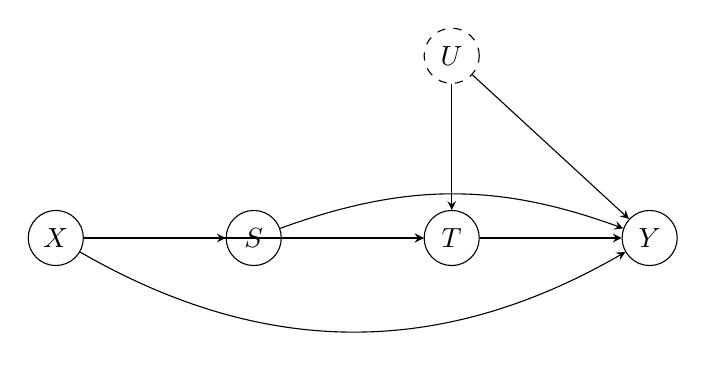
\begin{tikzpicture}[
  node distance=1.6cm and 1.8cm,
  roundnode/.style={circle, draw=black, minimum size=7mm, inner sep=0pt},
  latentnode/.style={circle, draw=black, dashed, minimum size=7mm, inner sep=0pt},
  >=stealth
]
  \node[roundnode] (X) {$X$};
  \node[roundnode, right=of X] (S) {$S$};
  \node[roundnode, right=of S] (T) {$T$};
  \node[roundnode, right=of T] (Y) {$Y$};
  \node[latentnode, above=of T] (U) {$U$};
  \draw[->] (X) -- (S);
  \draw[->] (X) -- (T);
  \draw[->] (X) to[bend right=30] (Y);
  \draw[->] (S) -- (T);
  \draw[->] (S) to[bend left=20] (Y);
  \draw[->] (T) -- (Y);
  \draw[->] (U) -- (T);
  \draw[->] (U) -- (Y);
\end{tikzpicture}
\caption{SCM for a single chess decision. $C=f(S)$ is not a separate node; it is
a deterministic encoding of $S$ used as an alternative covariate. We compare
adjustment on $(S,X)$, $(f(S),X)$, and $(Z,X)$ as competing encodings of the
same back-door problem.}
\label{fig:scm_chess}
\end{figure}

% -------------------------------------------------------
\section{Theory: Variance Reduction via Sufficient Encodings}
\label{sec:theory}
% -------------------------------------------------------

\paragraph{Setup.}
Let $X_{\text{adj}}\in\{(S,X),(C,X),(Z,X)\}$ index a candidate adjustment set,
with $C=AS$ for some $A\in\mathbb{R}^{k\times d}$, $k\ll d$. Assume
ignorability $(Y(0),Y(1))\perp T\mid S,X$, positivity
$0<P(T{=}1\mid S,X)<1$, and consistency throughout. Define the propensity and
outcome regression
\[
e(\cdot)=P(T{=}1\mid X_{\text{adj}}{=}\cdot),\qquad
\mu_t(\cdot)=\mathbb{E}[Y\mid T{=}t,X_{\text{adj}}{=}\cdot].
\]
Say $C$ is \emph{sufficient} for $S$ with respect to $(T,Y)$ given $X$ if
$(T,Y)\perp S\mid (C,X)$.

\begin{quote}
\textbf{Proposition (sufficient-encoding variance reduction).}
\emph{If $C$ is sufficient for $S$ given $X$, then (i) $\tau$ is identified
from $X_{\text{adj}}=(C,X)$; (ii) the semiparametric efficiency bound for
$\tau$ on $(C,X)$ equals the bound on $(S,X)$; and (iii) for any
nuisance learner whose $L^2$ rate is monotone in input dimension, the
finite-$N$ second-order error of the cross-fitted DR estimator on $(C,X)$ is
no larger than that on $(S,X)$, and is strictly smaller whenever the
nuisance learner has not yet reached its parametric rate at the relevant
input dimension.}
\end{quote}

\paragraph{Argument.}
Identification follows because $(T,Y)\perp S\mid (C,X)$ combined with
ignorability gives $(Y(0),Y(1))\perp T\mid (C,X)$. The efficient influence
function for $\tau$ depends only on the $\sigma$-field of covariates
sufficient for $(T,Y)$ given $X$,\cite{hahn1998role} so switching the
$\sigma$-field generator from $(S,X)$ to $(C,X)$ preserves the bound. For
the finite-sample part, a cross-fitted DR estimator
satisfies\cite{chernozhukov2018double}
\[
\hat\tau-\tau \;=\;\bar\varphi(P)+O_P\big(\|\hat e-e\|_{L^2}\,\|\hat\mu_t-\mu_t\|_{L^2}\big),
\]
and the leading product term shrinks when $\hat e,\hat\mu_t$ are estimated
on the lower-dimensional $(C,X)$ rather than $(S,X)$ for any
dimension-monotone $L^2$ rate (e.g.\ kernel, sieve, gradient-boosted
ensembles).\cite{ma2012semiparametric,nabi2022causal}

\paragraph{Three empirical predictions.}
The proposition predicts: (P1)~a small-$N$ advantage for concept-level
adjustment that closes as $N\to\infty$ when $C$ is exactly sufficient;
(P2)~when $C$ is only \emph{approximately} sufficient, raw $(S,X)$ overtakes
$(C,X)$ once the nuisance-estimation penalty has decayed and the residual
sufficiency gap dominates; and (P3)~learned $Z$ inherits part of the benefit
only to the extent that it recovers a sufficient reduction of $S$.
Sec.~\ref{sec:results} matches all three: P1 is the small-$N$ concept lead,
P2 is the large-$N$ raw crossover at $\gamma>0$, and P3 is the intermediate
profile of $X_{\text{learned}}$ traced to weak outcome-model fit. A full
proof is in Appendix~\ref{app:proof}.

% -------------------------------------------------------
\section{Experimental Setup}
% -------------------------------------------------------

\paragraph{Data.}
We extract ${\sim}30{,}000$ decision points from classical ($\geq 25$\,min)
rated ($>1800$ Elo) Lichess games, sampling up to 18 plies in $[10,120]$ per
game. For each position we compute three covariate encodings: a raw 1152-d
bitboard tensor $S$, a 12-d expert concept vector $C=f(S)$ (structural features
plus engine sub-terms\cite{stockfish}), and a 32-d learned embedding $Z$
(Sec.~``Learned representation'' below). All three are concatenated with a
shared 6-d context $X$.

\paragraph{Treatment and outcome.}
$T\in\{0,1\}$ is assigned by a rule-based aggression score $A(S,m)$ over
captures, checks, king-zone pressure, sacrifices, and retreats; engine
evaluation is excluded from $T$ by construction. Outcomes are semi-synthetic
with planted $\tau^*$:
$Y(0)=\varphi(X)+\psi(C)+\gamma U+\varepsilon_0$,\ $Y(1)=Y(0)+\tau^*$, where
$\psi(C)$ uses only structural concepts (material balance, king pawn shield;
no Stockfish total eval). Confounding is induced by $U\sim\mathcal{N}(0,1)$ at
strength $\gamma$ and a logit shift $\alpha U$ on $T$ ($\alpha=0.3$). We
report a homogeneous regime ($\tau^*=0.3$) and a heterogeneous regime
($\tau^*(X)=0.1+0.3\cdot\mathbf{1}\{\text{material}>0\}$).

\paragraph{Estimators.}
The primary estimator is a cross-fitted ($K=5$) Doubly Robust
Learner\cite{chernozhukov2018double} with a logistic-regression propensity and
a LightGBM outcome model. A T-Learner baseline and a DR-Learner with a linear
(Ridge) outcome are used for the robustness analysis. All three reuse the same
seeds so differences are attributable to the representation.

\paragraph{Learned representation.}
$Z$ is a linear deconfounding embedding\cite{kuang2020information,deconfoundingScores}:
standardize $[S;X]$, fit a regularised logistic propensity, project out the
treatment-discriminative direction, and PCA-compress the residual to 32
dimensions.

\paragraph{Grid.}
We sweep $N\in\{1\text{k},2\text{k},5\text{k},10\text{k},20\text{k}\}$,
$\gamma\in\{0,0.3,0.6\}$, both $\tau^*$ regimes, all three representations,
all three estimator configurations, and 10 seeds per cell (2{,}700 fits).
Implementation details, hyperparameters, and seeds are in
Appendix~\ref{app:repro}.

% -------------------------------------------------------
\section{Results}
\label{sec:results}
% -------------------------------------------------------

We report the canonical configuration (homogeneous $\tau^*=0.3$, $\gamma=0.3$,
$\alpha=0.3$, DR-Learner with LightGBM); full $\gamma$ and heterogeneous
results are in the appendix.

\paragraph{Three regime claims.}
\textbf{Claim 1 (small-$N$):} at $N<N^*(\gamma)$, $X_{\text{concept}}$ achieves
lower ATE error than $X_{\text{raw}}$ and $X_{\text{learned}}$ due to reduced
nuisance complexity. \textbf{Claim 2 (large-$N$ crossover):} at
$N\gg N^*(\gamma)$ and $\gamma>0$, $X_{\text{raw}}$ overtakes
$X_{\text{concept}}$, with $X_{\text{learned}}$ in between, reflecting an
asymptotic sufficiency gap in the 12-d expert basis.
\textbf{Claim 3 (robustness):} under nuisance-model misspecification
$X_{\text{concept}}$ is more stable than $X_{\text{raw}}$, with
$X_{\text{learned}}$ intermediate.

\subsection{H1: Sample Efficiency}
Fig.~\ref{fig:bias_vs_N} plots median ATE bias (with IQR over 10 seeds)
against $N$ across confounding levels. Both terms of the Sec.~\ref{sec:theory}
argument are visible in it. At small $N$, raw begins with
high bias (0.33 / 0.43 / 0.55 at $\gamma\in\{0,0.3,0.6\}$, $N{=}1{,}000$) while
concept and learned start near their large-$N$ values; at $N{=}2{,}000$,
$\gamma{=}0.3$, concept bias (0.083) is roughly half of raw (0.165),
confirming H1. As $N$ grows, raw drops monotonically while concept and learned
plateau at a $\gamma$-dependent floor; at $N{=}20{,}000$, $\gamma{=}0.3$, raw
(0.034) falls below concept (0.078) and learned (0.067), and similarly at
$\gamma{=}0.6$. At $\gamma{=}0$ no sufficiency gap exists and all three
converge to near zero. Where the crossover $N^{\text{cross}}(\gamma)$ falls
tells us how far the concept basis is from being a sufficient statistic.
Learned $Z$ never beats concept consistently and never catches raw at large
$N$; the nuisance diagnostics below trace this to weak outcome-model fit.
Numerical thresholds are in Appendix~\ref{app:t3}.

\begin{figure}[t]
\centering
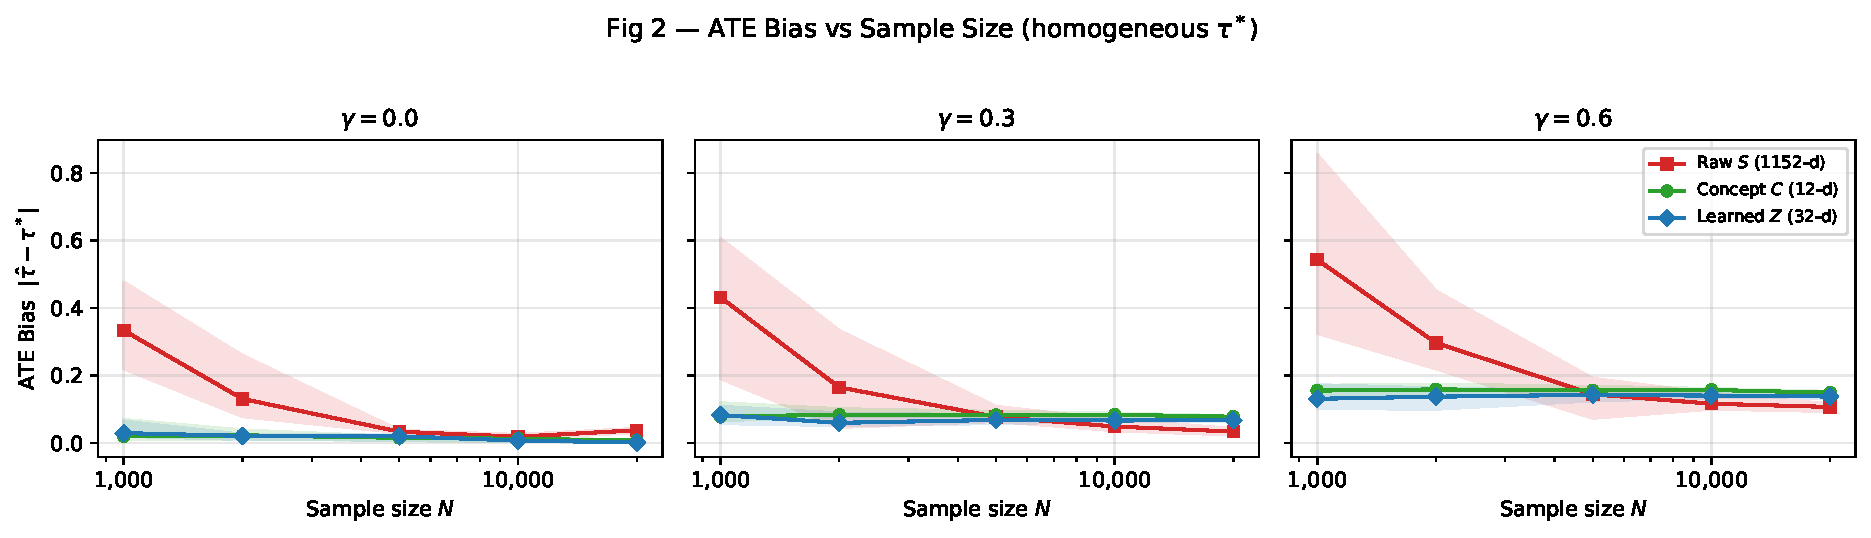
\includegraphics[width=\linewidth]{../pilot/outputs/figures/fig2_ate_bias_vs_N_homogeneous.pdf}
\caption{ATE bias $|\hat{\tau}-\tau^*|$ vs.\ $N$ for the three representations
under different confounding strengths $\gamma$. Median over 10 seeds; shading
shows IQR. The concept gap is widest at small $N$ (Claim~1); raw overtakes at
large $N$ once $\gamma>0$ (Claim~2).}
\label{fig:bias_vs_N}
\end{figure}

\paragraph{T3: sample-efficiency thresholds.}
Table~\ref{tab:t3-main} reports the smallest $N$ at which median ATE bias
first falls below a target $\epsilon$, by linear interpolation between
adjacent grid points (Task~T3 of the testbed). At $\gamma\in\{0,0.3\}$
concept and learned reach $\epsilon{=}0.10$ at the smallest grid point, while
raw needs 2--4$\times$ more data, which puts a number on H1. At
$\gamma{=}0.3$ and $\epsilon{=}0.05$ the ordering reverses. Concept and learned
hit the sufficiency-gap floor and never drop below 0.05 within the grid, while
raw does so at around $N\approx 9{,}775$. This is the Claim~2 crossover in
sample-size terms.

\begin{table}[t]
\caption{Sample-efficiency threshold $N_{T3}(\text{rep},\gamma,\epsilon)$:
smallest $N$ at which median ATE bias $\leq\epsilon$ over 10 seeds, canonical
setting (homogeneous $\tau^*$, DR-Learner with LightGBM outcome). ``$>$20k''
denotes a threshold not reached within the grid; ``$\leq$1k'' denotes a
threshold already met at the smallest grid point.}
\label{tab:t3-main}
\centering
\small
\begin{tabular}{lcccccc}
\toprule
 & \multicolumn{2}{c}{$\gamma=0$} & \multicolumn{2}{c}{$\gamma=0.3$} & \multicolumn{2}{c}{$\gamma=0.6$} \\
\cmidrule(lr){2-3}\cmidrule(lr){4-5}\cmidrule(lr){6-7}
Rep & $\epsilon{=}0.05$ & $\epsilon{=}0.10$ & $\epsilon{=}0.05$ & $\epsilon{=}0.10$ & $\epsilon{=}0.05$ & $\epsilon{=}0.10$ \\
\midrule
Raw $S$       & 4{,}486    & 2{,}945    & 9{,}775    & 4{,}223    & $>$20k & $>$20k \\
Concept $C$   & $\leq$1k   & $\leq$1k   & $>$20k     & $\leq$1k   & $>$20k & $>$20k \\
Learned $Z$   & $\leq$1k   & $\leq$1k   & $>$20k     & $\leq$1k   & $>$20k & $>$20k \\
\bottomrule
\end{tabular}
\end{table}

\subsection{H2: Nuisance-Model Robustness}
We swap the LightGBM outcome model for a linear Ridge model, holding the
propensity model fixed, at $N{=}2{,}000$, $\gamma{=}0.3$
(Fig.~\ref{fig:robustness}). Raw bias degrades from 0.165 to 0.261 (+58\%);
concept moves only from 0.082 to 0.077; learned stays near 0.06. This supports
H2 and Claim~3: with low-dimensional concept covariates, a less flexible model
is enough for an adequate fit.

\begin{figure}[t]
\centering
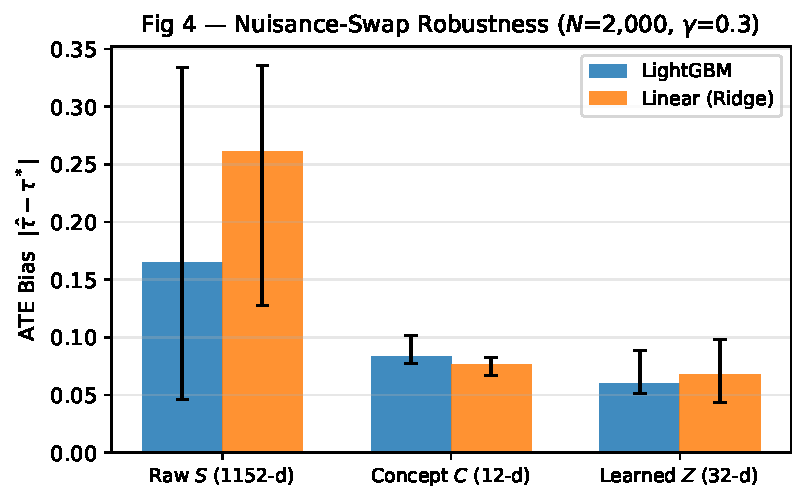
\includegraphics[width=0.7\linewidth]{../pilot/outputs/figures/fig4_robustness_homogeneous_g0.3.pdf}
\caption{Nuisance-swap robustness: ATE bias with LightGBM vs.\ linear outcome
model per representation ($N{=}2{,}000$, $\gamma{=}0.3$). Bars: median; error
bars: IQR over 10 seeds. Raw degrades $58\%$ on model swap; concept and
learned are stable.}
\label{fig:robustness}
\end{figure}

\subsection{Regime Diagram}
Fig.~\ref{fig:heatmap} shows ATE RMSE over the full $(\gamma,N)$ grid as a
heatmap per representation. Concept and learned dominate the high-$\gamma$,
low-$N$ corner (Claim~1); raw overtakes both in the high-$\gamma$, large-$N$
corner once the sufficiency gap dominates (Claim~2). The winner-per-cell
counterpart, with margins, is reported in Appendix~\ref{app:regime}.

\begin{figure}[t]
\centering
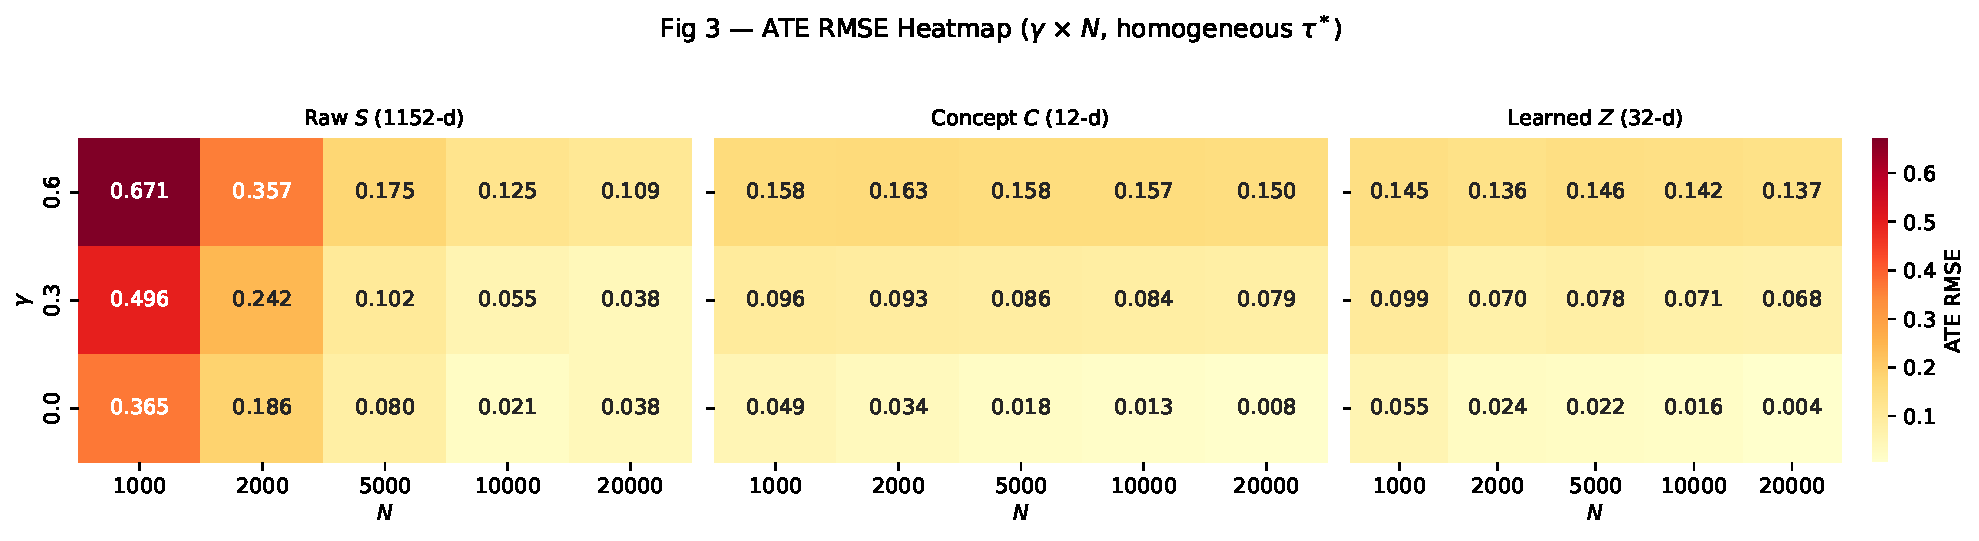
\includegraphics[width=\linewidth]{../pilot/outputs/figures/fig3_heatmap_homogeneous.pdf}
\caption{ATE RMSE over $(\gamma,N)$ per representation (DR-Learner, LightGBM).
Warmer colours: higher RMSE. Concept and learned dominate the high-$\gamma$,
low-$N$ corner; raw overtakes in the high-$\gamma$, large-$N$ corner.}
\label{fig:heatmap}
\end{figure}

\subsection{Bias--Variance Decomposition}
Fig.~\ref{fig:bv} splits the MSE of $\hat\tau$ across seeds into squared
bias and variance. At $\gamma{=}0.3$, raw's MSE at $N{=}1{,}000$ is almost
entirely variance, and it shrinks monotonically toward zero as $N$ grows.
Concept's MSE is mostly a flat $\text{Bias}^2$ floor that does not shrink with
more data. Both predictions from Sec.~\ref{sec:theory} appear in the same
plot: P1 (raw's variance penalty) and P2 (concept's sufficiency-gap floor). At
$\gamma{=}0.6$ the pattern repeats with a higher concept floor and a slower
drop in raw's variance, so raw wins at large $N$ where the gap is widest.
Learned $Z$ has lower $\text{Bias}^2$ than concept, since its 32-d residual
subspace captures part of the sufficiency gap, but its variance is much larger
and cancels most of that advantage.

\begin{figure}[t]
\centering
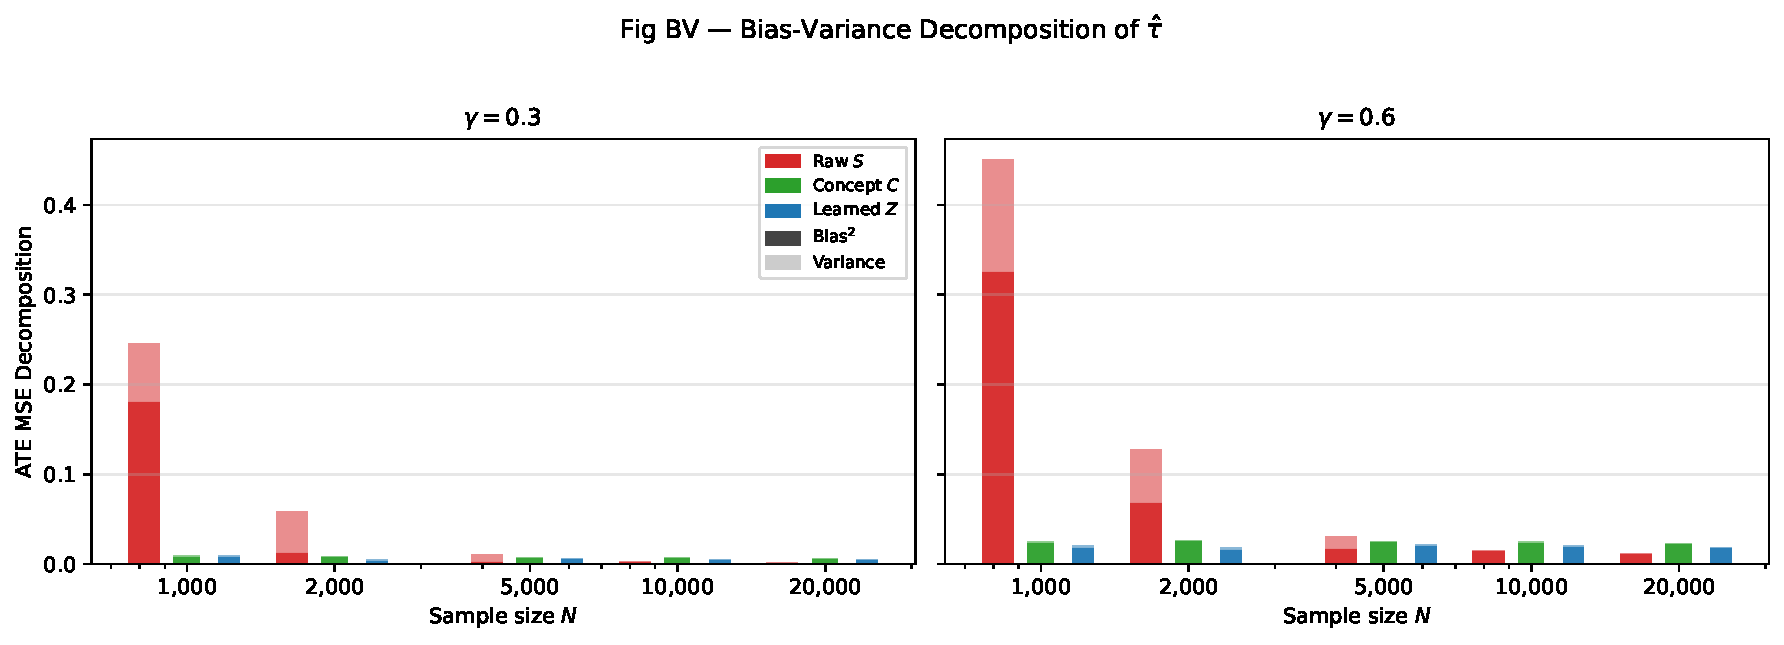
\includegraphics[width=\linewidth]{../pilot/outputs/figures/figBV.pdf}
\caption{Bias--variance decomposition of $\hat\tau$ at the canonical setting
(homogeneous $\tau^*$, DR-Learner with LightGBM outcome) at $\gamma{=}0.3$
(left) and $\gamma{=}0.6$ (right). Each bar stacks $\text{Bias}^2$ (dark) on
$\text{Variance}$ (light). Raw's large-$N$ advantage at $\gamma\geq 0.3$ is
mostly variance collapsing to zero; concept's plateau is a $\text{Bias}^2$
floor.}
\label{fig:bv}
\end{figure}

\subsection{Propensity Overlap and Nuisance Fit}
Fig.~\ref{fig:overlap} shows propensity-score histograms at $\gamma{=}0.6$,
$N{=}5{,}000$. Raw produces extreme propensities near 0 and 1 (pre-clip
minimum $\sim 10^{-7}$), violating positivity and destabilising the IPW
component of the DR estimator; concept maintains scores within
$[0.05,0.95]$; learned is in between. This explains raw's poor small-$N$
performance. With a high-dimensional adjustment set, the propensity model can
separate treated from control units almost perfectly, and IPW reweighting then
breaks down.

\begin{figure}[t]
\centering
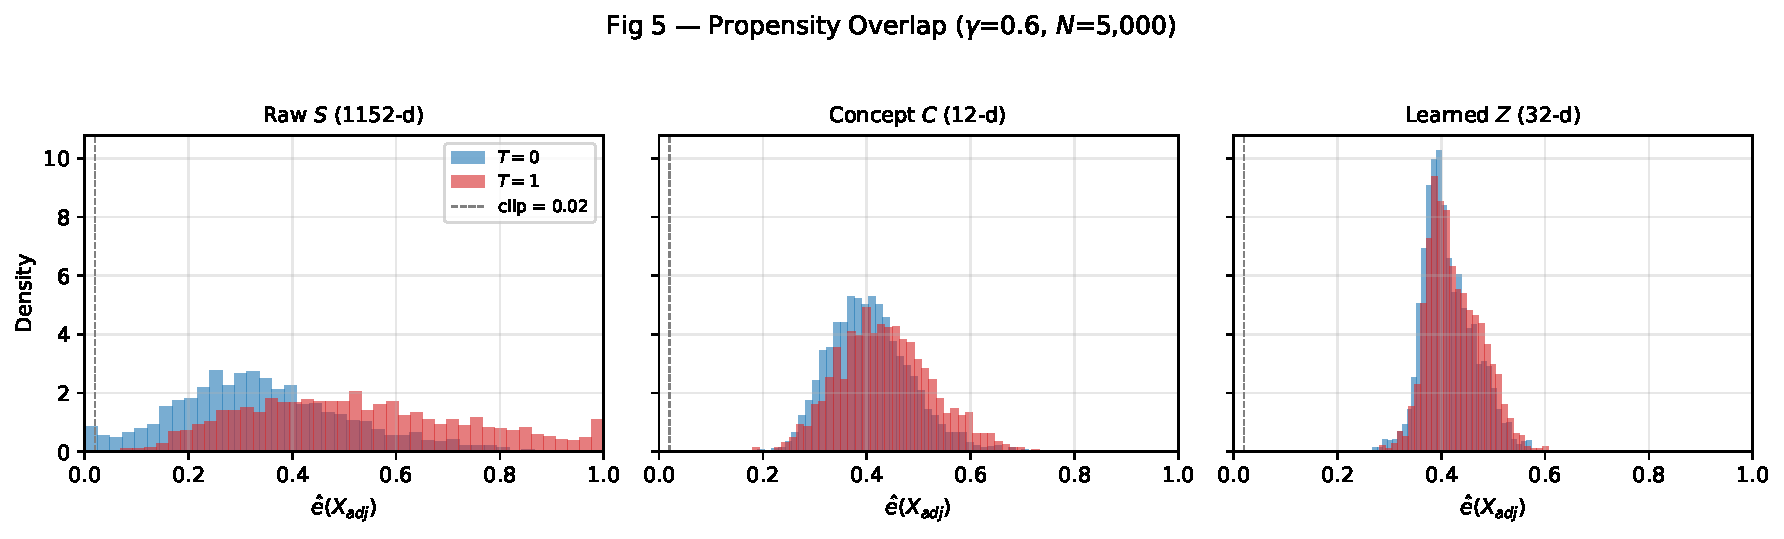
\includegraphics[width=\linewidth]{../pilot/outputs/figures/fig5_propensity_overlap_g0.6.pdf}
\caption{Propensity-score distributions $\hat{e}(X_{\text{adj}})$ per
representation at $\gamma{=}0.6$, $N{=}5{,}000$. Raw covariates produce
near-degenerate propensities; concept covariates maintain healthy overlap.
Dashed line: 0.02 clipping threshold.}
\label{fig:overlap}
\end{figure}

Nuisance-fit diagnostics show where the concept advantage comes from
(Fig.~\ref{fig:nuisance}). Concept consistently beats raw on
\emph{outcome} $R^2$ across the entire grid ($0.40\to 0.53$ for concept vs.\
$0.30\to 0.43$ for raw, $N\in[1\text{k},20\text{k}]$), but the propensity-AUC
gap is much smaller ($0.55\to 0.59$ for concept vs.\ $0.52\to 0.55$ for raw).
So the concept advantage comes mostly from the outcome model. A gradient-boosted
learner estimates $\mu_t(C,X)$ noticeably better than $\mu_t(S,X)$, while
$e(C,X)$ and $e(S,X)$ are about equally hard. Learned $Z$ has chance-level
outcome $R^2$ at every $N$ ($-0.10$ at $N{=}1{,}000$, $+0.04$ at
$N{=}20{,}000$), and its propensity AUC matches raw. In this DGP, the
unsupervised projection that defines $Z$ removes the outcome-predictive
directions. The resulting embedding is stable for IPW but useless for outcome
regression, which explains $Z$'s intermediate position in
Fig.~\ref{fig:bias_vs_N}.

\begin{figure}[t]
\centering
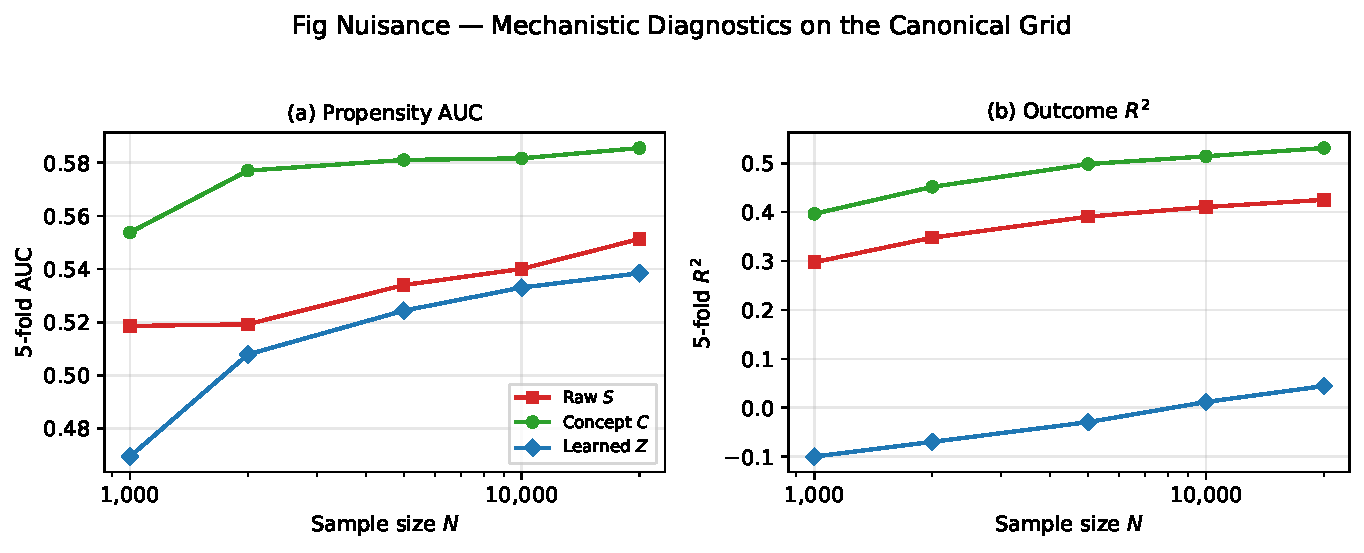
\includegraphics[width=\linewidth]{../pilot/outputs/figures/figNuisance.pdf}
\caption{Nuisance-model fit diagnostics at the canonical setting
($\gamma{=}0.3$, homogeneous~$\tau^*$, $N$ on log scale, 10-seed medians).
(a) 5-fold propensity AUC. (b) 5-fold outcome $R^2$. Concept dominates on
outcome fit, while all three reps have comparable propensity AUC; learned
$Z$ has chance-level outcome $R^2$.}
\label{fig:nuisance}
\end{figure}

\subsection{Concept-Level Causal Queries}
With $X_{\text{concept}}$, the stratifiers are already coordinates of $C$, so
conditional ATE queries over them are easy to pose.
Fig.~\ref{fig:qcate} reports three queries under the heterogeneous DGP at
$\gamma{=}0.3$, $N{=}5{,}000$, fit as stratified DR-Learners with the
stratifier passed as the heterogeneity feature: (Q1) CATE by material balance
$\{$behind, equal, ahead$\}$ (planted truths $\tau^*=0.1/0.1/0.4$); (Q2)
conditional ATE on the high-king-shield subset; (Q3) CATE by space-control
tercile (a false-positive check, since space is orthogonal to $\tau^*$).

Table~\ref{tab:q1-main} reports Q1 numerically. Concept recovers the planted
heterogeneity ($\hat\tau=0.178/0.183/0.515$, qualitatively matching
$0.1/0.1/0.4$) with SE $\approx 0.03$--$0.04$, roughly $10\times$ tighter
than raw's SE $\approx 0.18$--$0.42$. Raw gets the direction right, but its
confidence intervals are so wide that at $N{=}5{,}000$ the result cannot be
told apart from chance. On Q3, concept returns flat estimates
($0.232/0.239/0.284$ across terciles, SE $\sim 0.03$), while raw's stratum
estimates vary spuriously with SE $\sim 0.27$--$0.36$, so any heterogeneity
raw appears to find there is indistinguishable from sampling noise. Q2 (the
high-king-shield subset) is the only query where learned $Z$ has the lowest
bias. Appendix~\ref{app:qcate} traces this to the subset's stable material
distribution, which removes concept's usual outcome-side edge. Apart from Q2,
the pattern holds: concept-based adjustment gives interpretable conditional
effect estimates with usable variance, and 1152-d raw adjustment does not.

\begin{figure}[t]
\centering
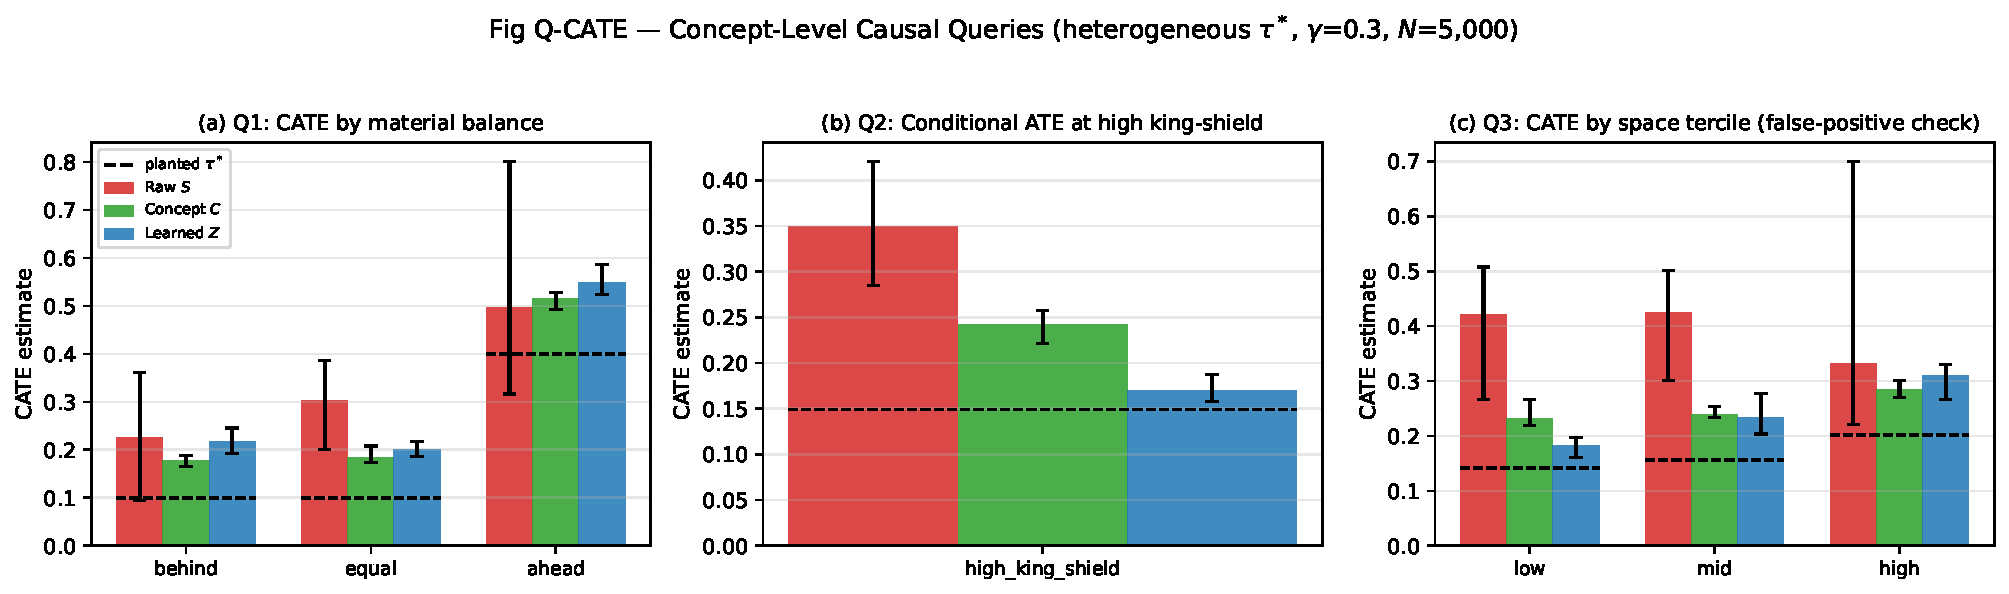
\includegraphics[width=\linewidth]{../pilot/outputs/figures/figQ_concept_queries.pdf}
\caption{Concept-level causal queries at $\gamma{=}0.3$, $N{=}5{,}000$,
heterogeneous $\tau^*$. (a) Q1: CATE by material balance, with planted
truths $\tau^*_{\text{behind,equal}}=0.1$ and $\tau^*_{\text{ahead}}=0.4$ as
dashed reference lines. (b) Q2: conditional ATE on the high-king-shield
subset. (c) Q3: CATE by space-control tercile (false-positive check). Bars:
median over 10 seeds; error bars: IQR.}
\label{fig:qcate}
\end{figure}

\begin{table}[t]
\caption{Q1: CATE by material balance. Heterogeneous $\tau^*$,
$\gamma{=}0.3$, $N{=}5{,}000$, median over 10 seeds. Planted truths:
$\tau^*_{\text{behind}}=\tau^*_{\text{equal}}=0.1$, $\tau^*_{\text{ahead}}=0.4$.}
\label{tab:q1-main}
\centering
\small
\begin{tabular}{llccc}
\toprule
Stratum & Rep & $\hat{\tau}$ & SE & $|\text{bias}|$ \\
\midrule
Behind ($m<-0.5$) & Raw     & $+0.225$ & $0.331$ & $0.153$ \\
                  & Concept & $+0.178$ & $0.036$ & $0.078$ \\
                  & Learned & $+0.218$ & $0.048$ & $0.118$ \\
\midrule
Equal ($|m|\leq0.5$) & Raw     & $+0.302$ & $0.182$ & $0.202$ \\
                     & Concept & $+0.183$ & $0.027$ & $0.083$ \\
                     & Learned & $+0.201$ & $0.034$ & $0.101$ \\
\midrule
Ahead ($m>0.5$) & Raw     & $+0.496$ & $0.423$ & $0.199$ \\
                & Concept & $+0.515$ & $0.041$ & $0.115$ \\
                & Learned & $+0.549$ & $0.054$ & $0.149$ \\
\bottomrule
\end{tabular}
\end{table}

\subsection{Oracle-Correlation Sanity Check}
Because both $C$ and the semi-synthetic $Y$ are partially derived from engine
computation, we re-run the pipeline with $Y$ replaced by the actual game
outcome (W/D/L $\to\{1,0.5,0\}$), a quantity with zero engine involvement.
Concept retains tighter ATE confidence intervals than raw across all sample
sizes (SE(raw)/SE(concept) $=7.64$ at $N{=}1{,}000$, $2.39$ at $N{=}10{,}000$),
so the concept advantage is not an artefact of oracle correlation. Full
ablation results are in Appendix~\ref{app:game-outcome}.

\paragraph{Secondary environment.}
We instantiate the same SCM/DGP protocol on a structured $10\times 10$
gridworld with a checkerboard parity confounder visible to $S$ but invisible
to $C$. The same qualitative regime structure replicates: concept wins at the
smallest $N$, raw overtakes once the finite-sample penalty decays, and learned
$Z$ underperforms throughout. Construction and full results are in
Appendix~\ref{app:gridworld}.

% -------------------------------------------------------
\section{Related Work}
% -------------------------------------------------------

\paragraph{Causal representations and concept models.}
Causal representation learning holds that representations aligned with the
underlying causal structure give models that are more robust, generalize
better, and support reasoning about interventions.\cite{scholkopf2021towards}
Concept Bottleneck Models (CBMs) route predictions through a human-meaningful
concept layer,\cite{koh2020concept} and structural or causally reliable
extensions add explicit causal constraints between concepts and
labels.\cite{fromCausalToConcept} These methods learn concepts end-to-end and
are evaluated on prediction. We instead treat $C$ as a fixed expert encoding
and evaluate it on \emph{causal} criteria (ATE accuracy, sample efficiency,
nuisance robustness). A CBM/SCBM bottleneck $h_\theta(S)$ fits into our
pipeline as a fourth representation.

\paragraph{Doubly-robust estimation and deconfounding embeddings.}
Cross-fitted DR estimation attains $\sqrt{N}$-asymptotic normality at
second-order remainder rates.\cite{chernozhukov2018double} At finite $N$, the
dimensionality of the nuisance inputs therefore becomes the limiting term,
which motivates the proposition in Sec.~\ref{sec:theory}.
Information-bottleneck and deconfounding-score
approaches\cite{kuang2020information,deconfoundingScores} try to learn
low-dimensional adjustment sets that approximate sufficient statistics; our
linear $Z$ is the simplest member of that family. Our diagnostics show one way
it fails. When a few features drive the propensity, the unsupervised
treatment-orthogonal projection also removes the most outcome-predictive
directions, and the embedding ends up stable for IPW but useless for outcome
regression.

\paragraph{Semiparametric efficiency and chess as a domain.}
Hahn\cite{hahn1998role} characterises the efficient influence function and
semiparametric bound for the ATE; Ma \& Zhu\cite{ma2012semiparametric} and
Nabi et al.\cite{nabi2022causal} extend these results under sufficient
dimension reduction, showing the bound is preserved while nuisance variance
decreases. Our proposition applies these results to cross-fitted DR. Chess has
been used before to study patterns, fortresses, and causal
models,\cite{lemeire2005causalmodelsinchess,fortressesPaper,causalMaskingSpatial}
usually without semi-synthetic potential outcomes or controlled confounding.
To our knowledge, \textsc{ChessCausalBench} is the first testbed in a strategic
game that combines a fully specified SCM, a planted ATE, adjustable $\gamma$,
and a plug-in interface for representations.

% -------------------------------------------------------
\section{Discussion and Limitations}
% -------------------------------------------------------

Chess and the gridworld give the same picture, and it matches the
linear-Gaussian theory. When data is scarce and confounding is non-trivial,
expert-defined concept representations are more sample-efficient and more
robust than high-dimensional raw encodings or our linear learned embedding. At
large $N$, raw encodings overtake them: their finite-sample nuisance-estimation
penalty has decayed, and the residual sufficiency gap of the concept basis is
what limits accuracy. Concepts compress the state into directions aligned with
the confounding structure, which improves overlap, lowers outcome-model
variance, and makes estimates less sensitive to model misspecification.

The concept-query results show a second effect of the representation that the
regime plot does not capture. Concept-based adjustment supports ``what-if''
questions over named features, such as isolating king safety while holding
material fixed. With 1152-d raw adjustment, the variance of such estimates is
too high to interpret. We take this as evidence that concept-level
abstractions act as \emph{structured causal pre-processing}: a pre-specified
inductive bias that reduces how much data is needed to learn useful
abstractions from raw state alone.

\paragraph{Practical takeaway and extensions.}
In practice, when $N$ is small or moderate and confounding is non-trivial, a
fixed expert encoding $C$ is the better default. Raw $(S,X)$ is preferable only
after the finite-sample nuisance penalty has decayed and a residual sufficiency
gap dominates. The crossover $N^{\text{cross}}(\gamma)$ measures how far $C$ is
from sufficient, and enriching the basis to push the crossover to larger $N$
is a natural extension of the testbed tasks. The learned-$Z$ results also show
how naive deconfounding can fail, so any embedding evaluated on the testbed
should be checked for outcome-model fit as well as propensity overlap.

\paragraph{Limitations.}
(i)~Our DGP plants outcomes that are linear in concepts, which may favour
concept-based adjustment; a non-linear outcome surface would stress all
representations more equally. (ii)~The linear deconfounding embedding is a
simplification and a non-linear variant might close more of the gap. (iii)~A
residual oracle-correlation pathway through Group~B engine sub-terms cannot be
fully excluded, though the game-outcome ablation argues it is not the dominant
effect. (iv)~Positivity violations at high $\gamma$ affect every representation
and our clipping mitigates but does not eliminate them. (v)~The gridworld
secondary environment is synthetic; validating the regime structure on a real
observational dataset is left to future work.

% -------------------------------------------------------
\bibliographystyle{plainnat}
\bibliography{refs}

\appendix

\section{Overview of Supplementary Material}
This appendix reports supplementary results referenced in the main text:
proof of the variance-reduction result, sample-efficiency thresholds (Task~T3),
bias-variance decomposition, the winner-per-cell regime diagram, crossover
analysis, nuisance-fit diagnostics, supervised residual compression
(closing the sufficiency gap), the concept-level causal queries Q1--Q3, the
game-outcome sanity ablation, the gridworld secondary environment, and
implementation details. All numbers are computed from the committed result
CSVs under \texttt{pilot/outputs/}; figure paths are under
\texttt{../pilot/outputs/figures/}.

% -------------------------------------------------------------------------
\section{Proof of the Sufficient-Encoding Variance-Reduction Result}
\label{app:proof}
\paragraph{Identification under sufficiency.}
Assume ignorability $(Y(0),Y(1))\perp T\mid S,X$, positivity, and consistency,
and assume $C=AS$ is sufficient for $S$ with respect to $(T,Y)$ given $X$:
$(T,Y)\perp S\mid C,X$. For any measurable $h$,
$\mathbb{E}[h(Y)\mid T,S,X]=\mathbb{E}[h(Y)\mid T,C,X]$ a.s., and similarly
$P(T\mid S,X)=P(T\mid C,X)$. Combining with ignorability gives
$(Y(0),Y(1))\perp T\mid C,X$, so $\tau$ is identified from observational data
under $X_{\text{adj}}=(C,X)$.

\paragraph{Efficiency bound.}
The efficient influence function for $\tau$ at law $P$ is, with
$e(x)=P(T{=}1\mid X_{\text{adj}}{=}x)$ and $\mu_t(x)=\mathbb{E}[Y\mid T{=}t,X_{\text{adj}}{=}x]$,
\[
\varphi(W;P)\;=\;\mu_1(X_{\text{adj}})-\mu_0(X_{\text{adj}})
+\frac{T(Y-\mu_1(X_{\text{adj}}))}{e(X_{\text{adj}})}
-\frac{(1-T)(Y-\mu_0(X_{\text{adj}}))}{1-e(X_{\text{adj}})}-\tau,
\]
and the semiparametric efficiency bound is $V^*(P)=\mathbb{E}[\varphi(W;P)^2]$.
Under sufficiency, $\mu_t$ and $e$ are functions of $(C,X)$ only, so
$\varphi$ is measurable with respect to $\sigma(C,X,T,Y)$; the bound based on
$(S,X)$ and the bound based on $(C,X)$ coincide.\cite{hahn1998role}

\paragraph{Finite-sample variance.}
A cross-fitted DR estimator $\hat\tau$ satisfies
$\sqrt{N}(\hat\tau-\tau)\overset{d}{\to}\mathcal{N}(0,V^*(P))$ provided the
nuisance estimators $\hat e,\hat\mu_t$ converge faster than
$N^{-1/4}$.\cite{chernozhukov2018double} The leading second-order term in the
error expansion is $O(\|\hat e-e\|_2\,\|\hat\mu_t-\mu_t\|_2)$, whose magnitude
depends on the dimensionality of the inputs to the nuisance estimators.
Estimating $e(c,x)$ and $\mu_t(c,x)$ over a $k$-dimensional $C$ rather than
$d$-dimensional $S$ reduces nuisance estimation error at any fixed $N$ for
standard $L^2$-rate-bounded learners (e.g., kernel, gradient boosting, sieve)
because the achievable rate scales with the effective input
dimension.\cite{ma2012semiparametric,nabi2022causal} Hence the finite-sample
variance of the DR estimator on $(C,X)$ is no larger than that on $(S,X)$ and
typically strictly smaller, while the asymptotic bound is identical.

\paragraph{Approximate sufficiency.}
If $C$ is only approximately sufficient, $(T,Y)\not\perp S\mid C,X$, the
variance argument still holds at finite $N$ but introduces an asymptotic bias
proportional to the residual conditional dependence. This is the source of the
empirical sufficiency gap that produces Claim~2.

% -------------------------------------------------------------------------
\section{Sample-Efficiency Threshold (Task T3)}
\label{app:t3}
Table~\ref{tab:t3} reports, for each representation and confounding level, the
smallest $N$ at which the median ATE bias first falls below a target
$\epsilon$ (linear interpolation between adjacent grid points).
``$>$20k'' means the threshold was not reached within the largest sample size
in the grid; ``$\leq$1k'' means the threshold was already met at the smallest
grid point. Fig.~\ref{fig:t3} visualises the same numbers on a log-scale bar
chart.

\begin{table}[h]
\caption{Sample-efficiency threshold $N_{T3}(\text{rep},\gamma,\epsilon)$:
smallest $N$ at which median ATE bias $\leq\epsilon$ over 10 seeds, canonical
setting (homogeneous $\tau^*$, DR-Learner with LightGBM outcome).}
\label{tab:t3}
\centering
\small
\begin{tabular}{lcccccc}
\toprule
 & \multicolumn{2}{c}{$\gamma=0$} & \multicolumn{2}{c}{$\gamma=0.3$} & \multicolumn{2}{c}{$\gamma=0.6$} \\
\cmidrule(lr){2-3}\cmidrule(lr){4-5}\cmidrule(lr){6-7}
Rep & $\epsilon{=}0.05$ & $\epsilon{=}0.10$ & $\epsilon{=}0.05$ & $\epsilon{=}0.10$ & $\epsilon{=}0.05$ & $\epsilon{=}0.10$ \\
\midrule
Raw $S$       & 4{,}486    & 2{,}945    & 9{,}775    & 4{,}223    & $>$20k & $>$20k \\
Concept $C$   & $\leq$1k   & $\leq$1k   & $>$20k     & $\leq$1k   & $>$20k & $>$20k \\
Learned $Z$   & $\leq$1k   & $\leq$1k   & $>$20k     & $\leq$1k   & $>$20k & $>$20k \\
\bottomrule
\end{tabular}
\end{table}

At $\gamma\in\{0,0.3\}$ concept and learned reach $\epsilon{=}0.10$ at the
smallest grid point while raw needs 2--4$\times$ more data. At $\gamma{=}0.3$
and $\epsilon{=}0.05$, concept and learned hit the sufficiency-gap floor and
never drop below 0.05 within the grid, while raw does (around
$N\approx 9{,}775$). At $\gamma{=}0.6$ no representation reaches
$\epsilon\leq 0.10$ within the grid.

\begin{figure}[h]
\centering
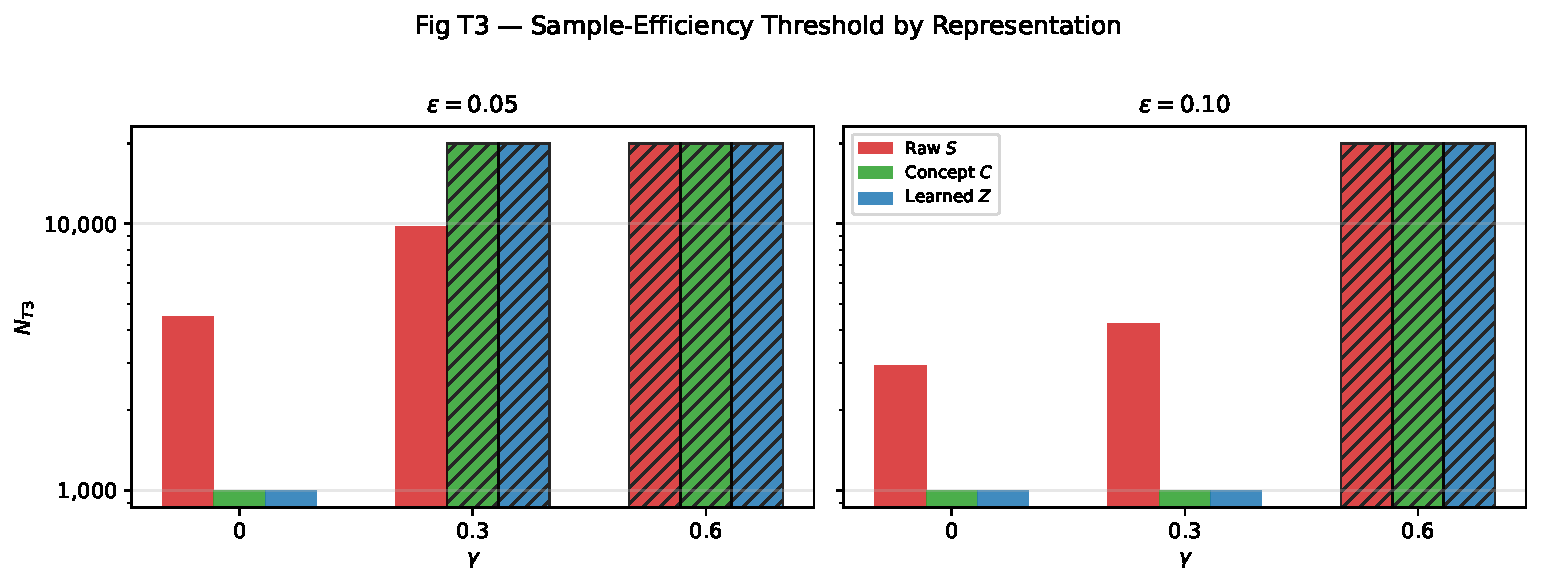
\includegraphics[width=\linewidth]{../pilot/outputs/figures/figT3.pdf}
\caption{Sample-efficiency threshold per representation and confounding level.
Two panels, one per target $\epsilon$. Hatched bars at $N{=}20{,}000$ indicate
cells where the threshold was not reached within the grid.}
\label{fig:t3}
\end{figure}

% -------------------------------------------------------------------------
\section{Bias--Variance Decomposition}
\label{app:bv}
Fig.~\ref{fig:bv-app} splits the MSE of each DR-Learner fit into squared bias
and variance across seeds. The decomposition is exact: for every
cell $\text{MSE}=\text{Bias}^2+\text{Var}$ to machine precision under a
population-variance estimator.

\begin{figure}[h]
\centering
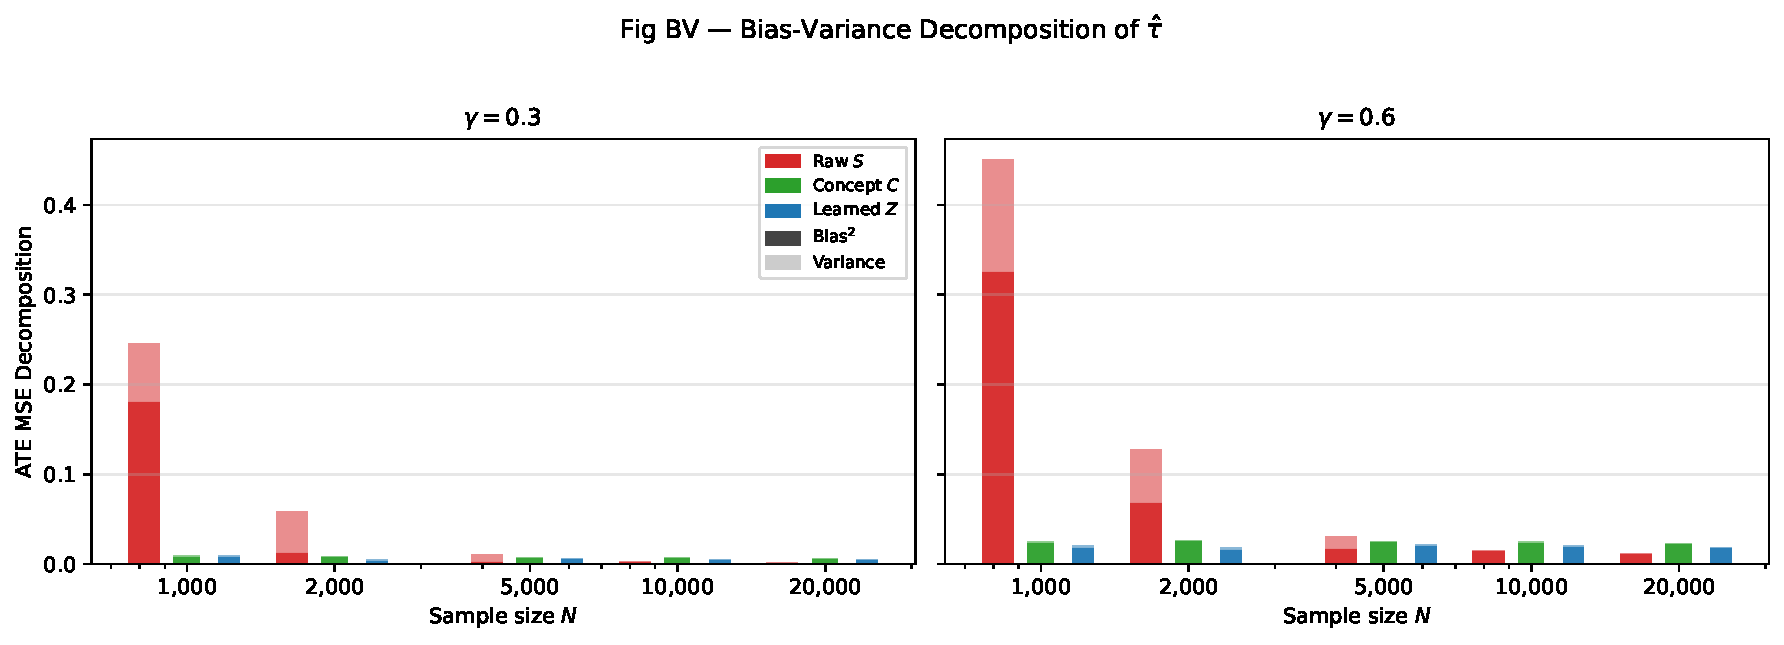
\includegraphics[width=\linewidth]{../pilot/outputs/figures/figBV.pdf}
\caption{Bias-variance decomposition of $\hat\tau$ at the canonical setting
(homogeneous $\tau^*$, DR-Learner with LightGBM outcome) at $\gamma{=}0.3$
(left) and $\gamma{=}0.6$ (right). Each bar stacks $\text{Bias}^2$ (dark) on
$\text{Variance}$ (light). Raw's large-$N$ advantage at $\gamma\geq 0.3$ is
mostly variance collapsing to zero; concept's plateau is a $\text{Bias}^2$
floor.}
\label{fig:bv-app}
\end{figure}

% -------------------------------------------------------------------------
\section{Winner-Per-Cell Regime Diagram}
\label{app:regime}
Fig.~\ref{fig:regime-app} shows the winning representation in each
$(\gamma,N)$ cell, with colour saturation encoding margin over the
second-best (darker = more decisive). Both $\tau^*$ regimes are shown.
Table~\ref{tab:regime} gives the exact margins for the homogeneous regime at
DR-LightGBM, the canonical main-paper setting.

\begin{figure}[h]
\centering
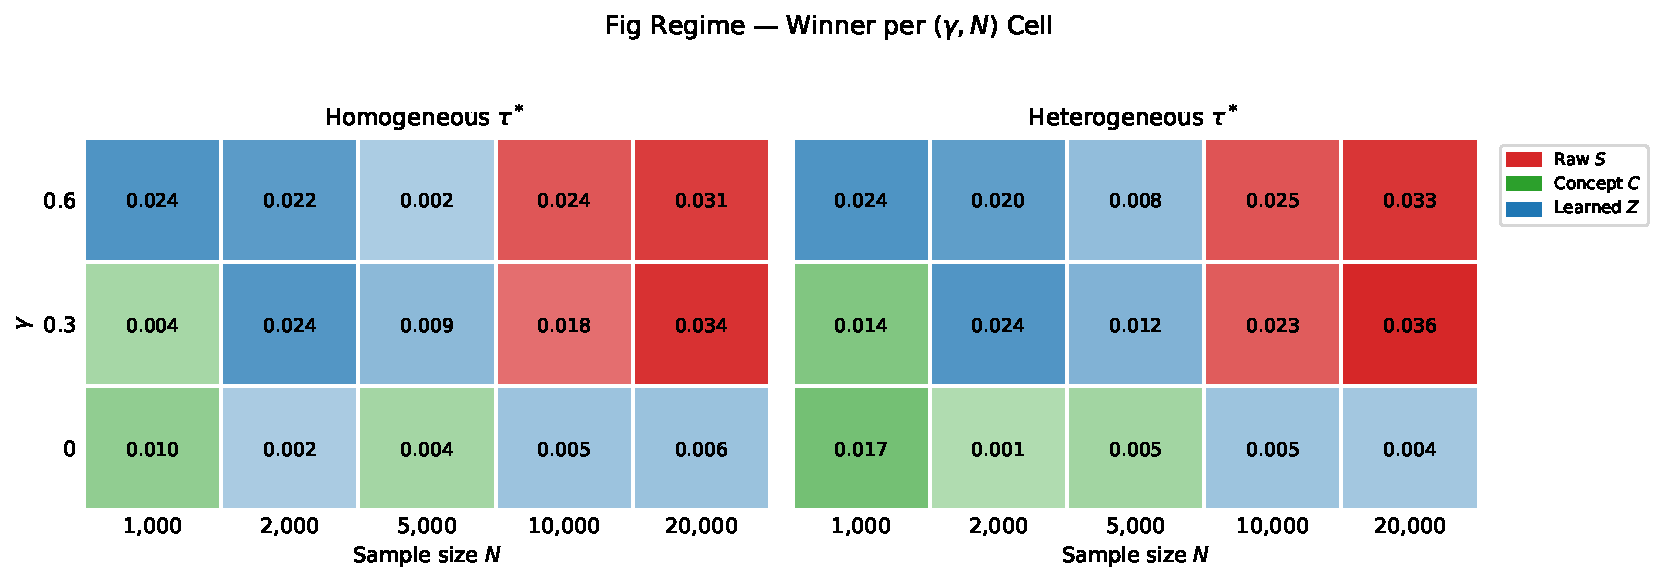
\includegraphics[width=\linewidth]{../pilot/outputs/figures/figRegime.pdf}
\caption{Winner-per-cell regime diagram over $(\gamma,N)$ for both $\tau^*$
regimes. Colour: winning representation; intensity: margin over second-best.}
\label{fig:regime-app}
\end{figure}

\begin{table}[h]
\caption{Winner per $(\gamma,N)$ cell, homogeneous $\tau^*$, DR-Learner with
LightGBM outcome. Margin = winner's median bias minus second-best's median
bias across 10 seeds.}
\label{tab:regime}
\centering
\small
\begin{tabular}{rlllll}
\toprule
$\gamma$ & $N{=}1{,}000$ & $N{=}2{,}000$ & $N{=}5{,}000$ & $N{=}10{,}000$ & $N{=}20{,}000$ \\
\midrule
0.0 & concept (0.010) & learned (0.002) & concept (0.004) & learned (0.005) & learned (0.006) \\
0.3 & concept (0.004) & learned (0.023) & learned (0.009) & raw (0.018)     & raw (0.034)     \\
0.6 & learned (0.024) & learned (0.022) & learned (0.002) & raw (0.024)     & raw (0.031)     \\
\bottomrule
\end{tabular}
\end{table}

% -------------------------------------------------------------------------
\section{Crossover-Point Analysis}
\label{app:crossover}
Table~\ref{tab:crossover} gives the empirical crossover sample size
$N^{\text{cross}}(\gamma)$ at which one representation's median bias curve
intersects another, by linear interpolation in $\log N$ between adjacent grid
points. Fig.~\ref{fig:cross} plots the same values as a function of $\gamma$.

\begin{table}[h]
\caption{Crossover points between representation pairs, homogeneous $\tau^*$,
DR-Learner with LightGBM outcome.}
\label{tab:crossover}
\centering
\small
\begin{tabular}{rlll}
\toprule
$\gamma$ & Raw vs.\ Concept & Raw vs.\ Learned & Learned vs.\ Concept \\
\midrule
0.0 & $>$20k & $>$20k & $N^{\text{cross}}\approx 1{,}807$ \\
0.3 & $N^{\text{cross}}\approx 4{,}713$ & $N^{\text{cross}}\approx 6{,}315$ & $N^{\text{cross}}\approx 1{,}107$ \\
0.6 & $N^{\text{cross}}\approx 4{,}669$ & $N^{\text{cross}}\approx 5{,}216$ & $<$1k \\
\bottomrule
\end{tabular}
\end{table}

\begin{figure}[h]
\centering
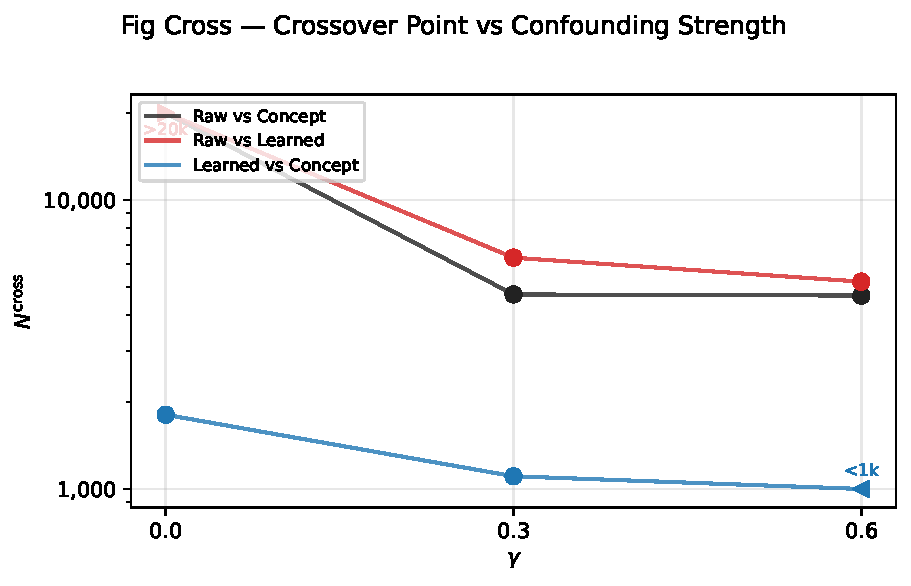
\includegraphics[width=0.7\linewidth]{../pilot/outputs/figures/figCross.pdf}
\caption{Crossover point $N^{\text{cross}}(\gamma)$ for each pair of
representations, homogeneous $\tau^*$. Right-arrow markers denote pairs that
never crossed within $N\leq 20{,}000$.}
\label{fig:cross}
\end{figure}

% -------------------------------------------------------------------------
\section{Nuisance-Fit Diagnostics}
\label{app:nuisance}
Fig.~\ref{fig:nuisance-app} reports cross-validated propensity AUC and outcome
$R^2$ at the canonical setting. Concept dominates raw on outcome $R^2$ across
$N\in[1\text{k},20\text{k}]$ ($0.40\to 0.53$ vs.\ $0.30\to 0.43$); the
propensity-AUC gap is much smaller. Learned $Z$ has chance-level outcome $R^2$
at every $N$ ($-0.10$ at $N{=}1{,}000$, $+0.04$ at $N{=}20{,}000$) because the
unsupervised projection that defines $Z$ removes outcome-predictive directions
when the propensity is driven cleanly by a small number of features.

\begin{figure}[h]
\centering
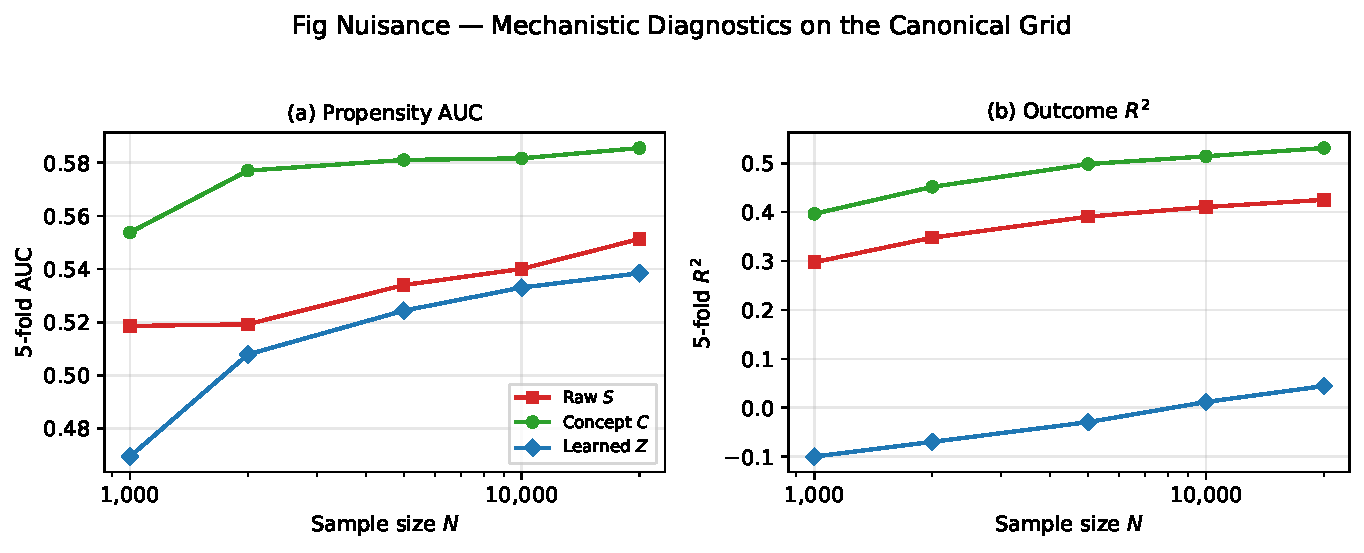
\includegraphics[width=\linewidth]{../pilot/outputs/figures/figNuisance.pdf}
\caption{Nuisance-model fit diagnostics at the canonical setting
($\gamma{=}0.3$, homogeneous~$\tau^*$, $N$ on log scale, 10-seed medians).
(a) 5-fold propensity AUC per representation. (b) 5-fold outcome $R^2$.
Concept dominates on outcome fit; the learned embedding $Z$ has chance-level
outcome $R^2$, which explains its intermediate position in the main
ATE-bias results.}
\label{fig:nuisance-app}
\end{figure}

% -------------------------------------------------------------------------
\section{Closing the Sufficiency Gap: Supervised Residual Compression}
\label{app:conplus}
If the sufficiency-gap interpretation is right, adding a compressed residual of
$S$ to the concept basis should help. We first try a variance-preserving
compression (\texttt{conplus\_pca}): linearly regress $S$ on $C$, reduce the
residual to 16 dimensions with PCA, and adjust on
$[C,\mathrm{PCA}_{16}(S-\widehat{E}[S\mid C]),X]$. This does not help; the
result tracks the concept curve almost exactly (Fig.~\ref{fig:conplus}).
Replacing PCA with a $T$-supervised partial least squares projection
(\texttt{conplus\_tpls}), which keeps the 16 directions with the highest
covariance with $T_{\text{obs}}$, behaves differently at different $N$. At
small $N$ the extra dimensions cost more than they save ($0.104$ vs.\ concept
$0.079$ at $N{=}1{,}000$, $\gamma{=}0.3$). In the mid-range T-PLS edges out
concept and approaches raw ($0.075$ vs.\ raw $0.077$ at $N{=}5{,}000$,
$\gamma{=}0.3$). At large $N$ it converges back toward concept, and raw keeps
a margin. The missing information is therefore not in the high-variance
residual directions, since PCA fails. Part of it lies in treatment-discriminative
residual directions, which T-PLS partly recovers, but no fixed-dimension
linear supervised residual captures all of it at the dimensions we tested.

\begin{figure}[h]
\centering
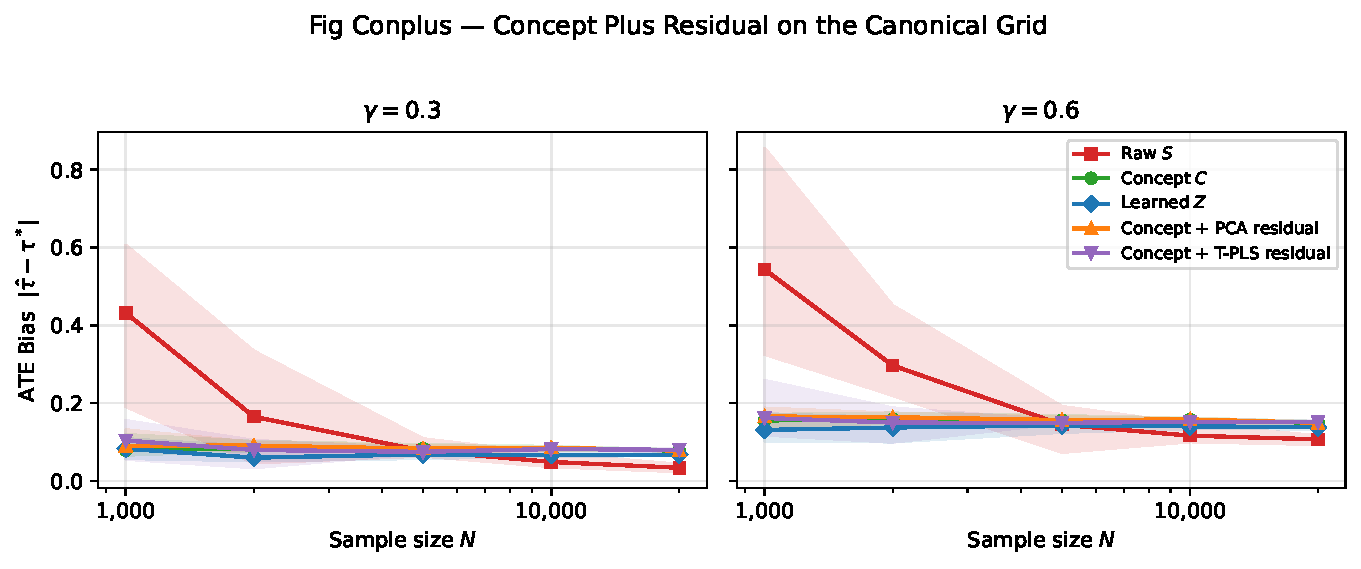
\includegraphics[width=\linewidth]{../pilot/outputs/figures/figConplus.pdf}
\caption{Residual augmentation on the canonical chess grid (homogeneous
$\tau^*$, DR-Learner, LightGBM). Orange: concept plus PCA residual (negative
control, tracks concept). Purple: concept plus $T$-supervised PLS residual,
which improves over concept across the mid-range without fully recovering raw.}
\label{fig:conplus}
\end{figure}

% -------------------------------------------------------------------------
\section{Concept-Level Causal Queries (Q-CATE)}
\label{app:qcate}
Fig.~\ref{fig:qcate-app} reports recovered CATE per stratum for the three queries
defined in the main text, under heterogeneous $\tau^*(X)=0.1+0.3\cdot
\mathbf{1}\{\text{material}>0\}$ at $\gamma{=}0.3$, $\alpha{=}0.3$, $N{=}5{,}000$,
10 seeds. Tables~\ref{tab:q1}--\ref{tab:q3} give numerical summaries.

\begin{figure}[h]
\centering
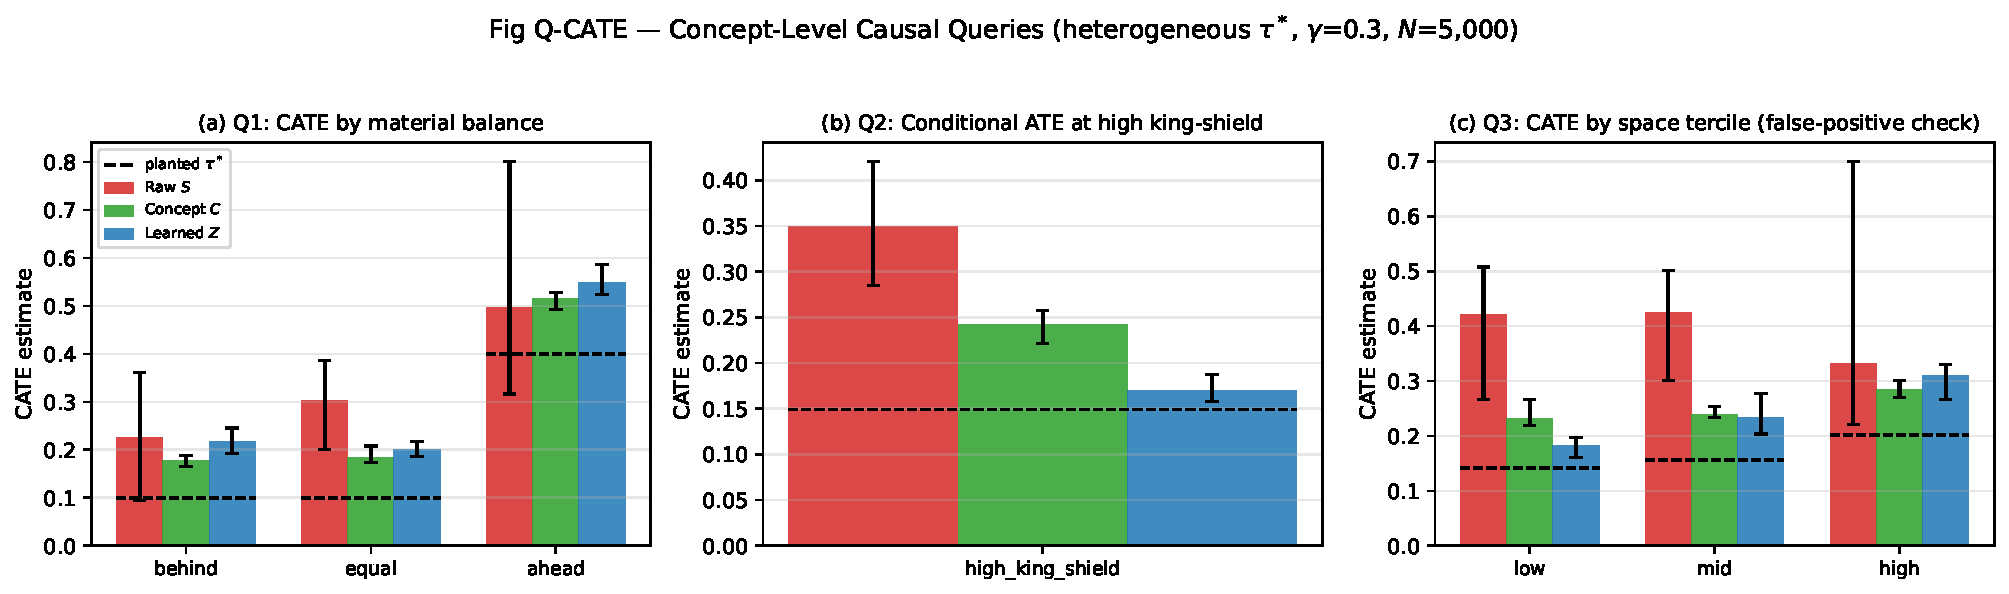
\includegraphics[width=\linewidth]{../pilot/outputs/figures/figQ_concept_queries.pdf}
\caption{Concept-level causal queries. (a) Q1: CATE by material balance, with
planted truths $\tau^*_{\text{behind,equal}}=0.1$ and
$\tau^*_{\text{ahead}}=0.4$ as dashed reference lines. (b) Q2: conditional ATE
on the high-king-shield subset. (c) Q3: CATE by space-control tercile
(false-positive check). Bars: median over 10 seeds; error bars: IQR.}
\label{fig:qcate-app}
\end{figure}

\begin{table}[h]
\caption{Q1: CATE by material balance. Heterogeneous $\tau^*$,
$\gamma=0.3$, $N=5{,}000$, median over 10 seeds. Planted truths:
$\tau^*_{\text{behind}}{=}\tau^*_{\text{equal}}{=}0.1$,
$\tau^*_{\text{ahead}}{=}0.4$.}
\label{tab:q1}
\centering
\small
\begin{tabular}{llcccc}
\toprule
Stratum & Rep & $\hat{\tau}$ & SE & $|\text{bias}|$ & $n_{\text{sub}}$ \\
\midrule
Behind ($m<-0.5$) & Raw      & $+0.225$ & $0.331$ & $0.153$ & 1{,}571 \\
                   & Concept  & $+0.178$ & $0.036$ & $0.078$ & 1{,}571 \\
                   & Learned  & $+0.218$ & $0.048$ & $0.118$ & 1{,}571 \\
\midrule
Equal ($|m|\leq0.5$) & Raw      & $+0.302$ & $0.182$ & $0.202$ & 2{,}358 \\
                     & Concept  & $+0.183$ & $0.027$ & $0.083$ & 2{,}358 \\
                     & Learned  & $+0.201$ & $0.034$ & $0.101$ & 2{,}358 \\
\midrule
Ahead ($m>0.5$)    & Raw      & $+0.496$ & $0.423$ & $0.199$ & 1{,}063 \\
                   & Concept  & $+0.515$ & $0.041$ & $0.115$ & 1{,}063 \\
                   & Learned  & $+0.549$ & $0.054$ & $0.149$ & 1{,}063 \\
\bottomrule
\end{tabular}
\end{table}

\begin{table}[h]
\caption{Q2: conditional ATE restricted to positions with
$c_{\text{king\_shield}}\geq$ 75th percentile. Conditional query, not
$do(c_{\text{king\_shield}}=\text{high})$.}
\label{tab:q2}
\centering
\small
\begin{tabular}{lcccc}
\toprule
Rep & $\hat{\tau}$ & SE & $|\text{bias}|$ & $n_{\text{sub}}$ \\
\midrule
Raw     & $+0.349$ & $0.258$ & $0.236$ & 1{,}733 \\
Concept & $+0.243$ & $0.037$ & $0.093$ & 1{,}733 \\
Learned & $+0.170$ & $0.044$ & $0.026$ & 1{,}733 \\
\bottomrule
\end{tabular}
\end{table}

\begin{table}[h]
\caption{Q3: CATE by space-control tercile (false-positive check).}
\label{tab:q3}
\centering
\small
\begin{tabular}{llcccc}
\toprule
Stratum & Rep & $\hat{\tau}$ & SE & $|\text{bias}|$ & $n_{\text{sub}}$ \\
\midrule
Low  & Raw     & $+0.421$ & $0.313$ & $0.325$ & 1{,}793 \\
     & Concept & $+0.232$ & $0.034$ & $0.090$ & 1{,}793 \\
     & Learned & $+0.182$ & $0.046$ & $0.041$ & 1{,}793 \\
\midrule
Mid  & Raw     & $+0.424$ & $0.272$ & $0.268$ & 1{,}774 \\
     & Concept & $+0.239$ & $0.032$ & $0.084$ & 1{,}774 \\
     & Learned & $+0.234$ & $0.043$ & $0.077$ & 1{,}774 \\
\midrule
High & Raw     & $+0.332$ & $0.355$ & $0.293$ & 1{,}423 \\
     & Concept & $+0.284$ & $0.036$ & $0.080$ & 1{,}423 \\
     & Learned & $+0.311$ & $0.051$ & $0.110$ & 1{,}423 \\
\bottomrule
\end{tabular}
\end{table}

% -------------------------------------------------------------------------
\section{Game-Outcome Sanity Ablation}
\label{app:game-outcome}
We replace $Y_{\text{obs}}$ with the actual game outcome from the side-to-move
perspective (W/D/L $\to\{1,0.5,0\}$), which has zero Stockfish involvement.
Fig.~\ref{fig:ablation} and Table~\ref{tab:ablation} report 240 fits across
$N\in\{1{,}000,2{,}000,5{,}000,10{,}000\}$, three representations, 10 seeds.
The SE ratio SE(raw)/SE(concept) is $7.64$ at $N{=}1{,}000$, $7.62$ at
$N{=}2{,}000$, $4.10$ at $N{=}5{,}000$, and $2.39$ at $N{=}10{,}000$. Because
the outcome variable now has no engine involvement, this advantage cannot be
explained by oracle correlation between concepts and the DGP.

\begin{figure}[h]
\centering
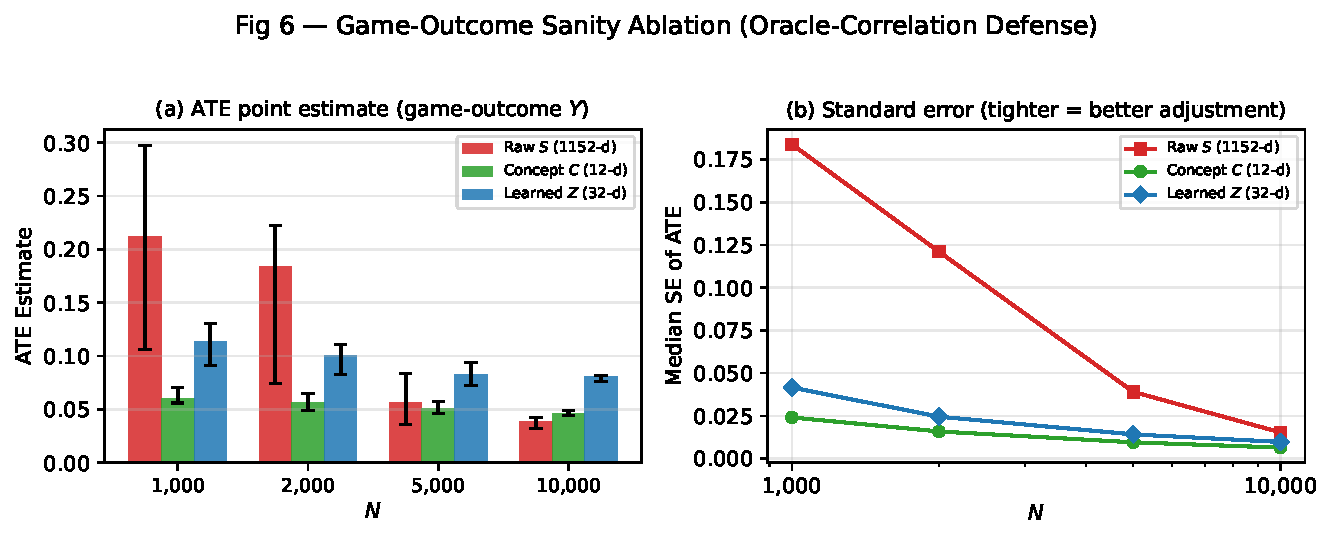
\includegraphics[width=\linewidth]{../pilot/outputs/figures/fig6_ablation_game_outcome.pdf}
\caption{Game-outcome sanity ablation. (a) ATE estimate per representation
across $N$ (median with IQR). (b) Median standard error of the ATE per
representation on a log-scale axis.}
\label{fig:ablation}
\end{figure}

\begin{table}[h]
\caption{Game-outcome ablation: DR-LightGBM ATE estimates and standard errors
per representation, with relative efficiency ratio SE(raw)/SE(concept).
Medians over 10 seeds.}
\label{tab:ablation}
\centering
\small
\begin{tabular}{rcccccccc}
\toprule
 & \multicolumn{2}{c}{Raw $S$} & \multicolumn{2}{c}{Concept $C$} & \multicolumn{2}{c}{Learned $Z$} & SE ratio \\
\cmidrule(lr){2-3}\cmidrule(lr){4-5}\cmidrule(lr){6-7}
$N$ & $\hat{\tau}$ & SE & $\hat{\tau}$ & SE & $\hat{\tau}$ & SE & raw/concept \\
\midrule
1{,}000  & $+0.212$ & $0.184$ & $+0.061$ & $0.024$ & $+0.114$ & $0.042$ & $\mathbf{7.64}$ \\
2{,}000  & $+0.184$ & $0.121$ & $+0.057$ & $0.016$ & $+0.100$ & $0.025$ & $\mathbf{7.62}$ \\
5{,}000  & $+0.057$ & $0.039$ & $+0.051$ & $0.010$ & $+0.082$ & $0.014$ & $\mathbf{4.10}$ \\
10{,}000 & $+0.039$ & $0.015$ & $+0.047$ & $0.006$ & $+0.081$ & $0.010$ & $\mathbf{2.39}$ \\
\bottomrule
\end{tabular}
\end{table}

% -------------------------------------------------------------------------
\section{Gridworld Secondary Environment}
\label{app:gridworld}
The gridworld is a $10\times10$ grid with obstacles and a goal: $S$ is a
$300$-d one-hot encoding (agent position, obstacle mask, goal position); $C$
is a 3-d expert vector (L1 distance to goal, local obstacle density, current
quadrant); $X$ is a 4-d context (step, seed, difficulty, start-distance);
$Z$ is the same linear deconfounding embedding as in chess. Treatment is a
calibrated sigmoid of
\[
\text{score}(S,X)=0.9\,d_z+0.8\,\rho_z+0.35\,\delta_z+0.15\,s_z-0.10\,k_z+1.0\,\chi_z,
\]
where $d$ is distance-to-goal, $\rho$ is local obstacle density, $\delta$ is
difficulty, $s$ is start-distance, $k$ is step number, and
$\chi(S)=(r+c)\bmod 2$ is the checkerboard parity of the agent cell;
subscript $z$ marks a standardized copy. The outcome DGP is
\[
Y(0)=0.4\,\delta_z+0.2\,s_z+0.1\,k_z+0.3\,d_z+0.2\,\rho_z+0.5\,\chi_z+\gamma U+\varepsilon_0,
\qquad Y(1)=Y(0)+\tau^*,
\]
with $\tau^*=0.3$, $U\sim\mathcal{N}(0,1)$,
$\varepsilon_0\sim\mathcal{N}(0,0.5^2)$, and a logit shift $\alpha_U=0.3$ on
$T_{\text{obs}}$. The parity $\chi$ is not in $C$, but it can be recovered
from the one-hot $S$, so the checker term is a confounder that is always
present and visible only through $S$. Here $\gamma$ therefore sets the strength
of \emph{additional} latent confounding on top of the checker baseline.

\begin{figure}[h]
\centering
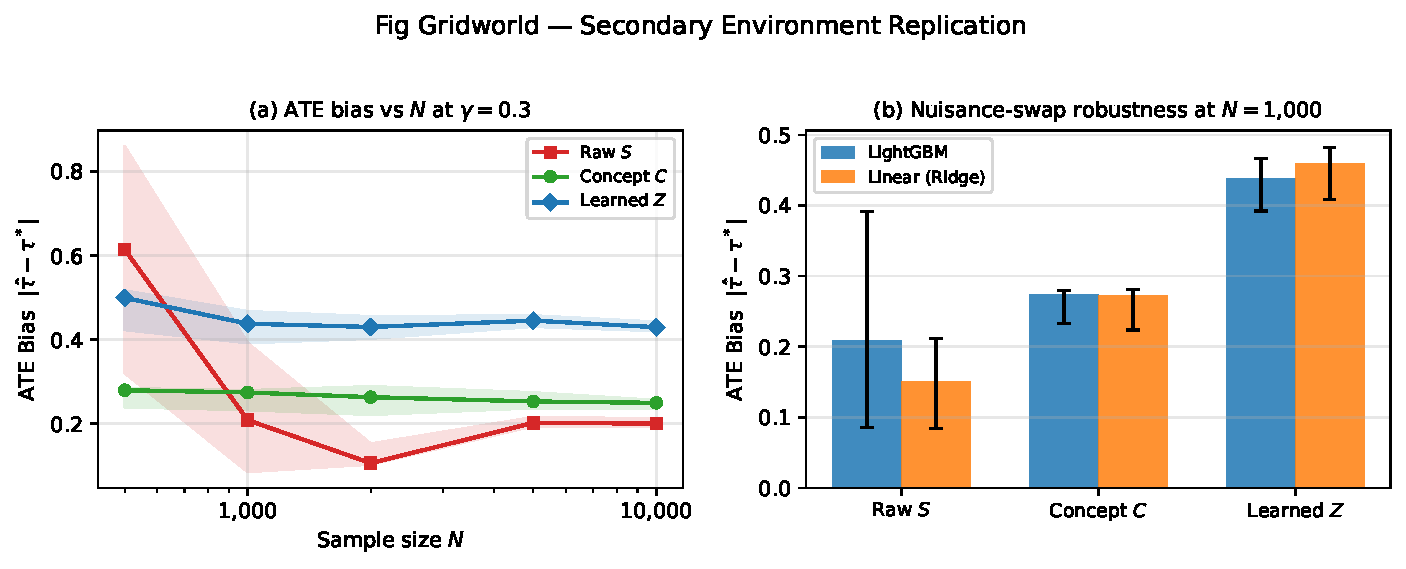
\includegraphics[width=\linewidth]{../pilot/outputs/figures/figGridworld.pdf}
\caption{Gridworld replication. (a) ATE bias vs.\ $N$ at $\gamma=0.3$.
(b) Nuisance-swap robustness bar chart at $N{=}1{,}000$, $\gamma=0.3$.
Concept wins at the smallest $N$, raw overtakes at larger $N$, learned $Z$
underperforms throughout.}
\label{fig:gridworld-app}
\end{figure}

\begin{table}[h]
\caption{Gridworld median ATE bias over 10 seeds, homogeneous $\tau^*$,
DR-Learner with LightGBM outcome. Bold: per-cell winner.}
\label{tab:gridworld}
\centering
\small
\begin{tabular}{rrrrr}
\toprule
$\gamma$ & $N$ & Raw & Concept & Learned \\
\midrule
0.0 & 500     & $0.540$           & $\mathbf{0.183}$  & $0.402$ \\
0.0 & 1{,}000 & $0.292$           & $\mathbf{0.204}$  & $0.362$ \\
0.0 & 2{,}000 & $\mathbf{0.047}$  & $0.185$           & $0.368$ \\
0.0 & 5{,}000 & $\mathbf{0.136}$  & $0.183$           & $0.383$ \\
0.0 & 10{,}000& $\mathbf{0.136}$  & $0.176$           & $0.365$ \\
\midrule
0.3 & 500     & $0.615$           & $\mathbf{0.280}$  & $0.499$ \\
0.3 & 1{,}000 & $\mathbf{0.209}$  & $0.274$           & $0.438$ \\
0.3 & 2{,}000 & $\mathbf{0.106}$  & $0.263$           & $0.430$ \\
0.3 & 5{,}000 & $\mathbf{0.202}$  & $0.253$           & $0.445$ \\
0.3 & 10{,}000& $\mathbf{0.200}$  & $0.250$           & $0.430$ \\
\midrule
0.6 & 500     & $0.580$           & $\mathbf{0.354}$  & $0.518$ \\
0.6 & 1{,}000 & $\mathbf{0.276}$  & $0.326$           & $0.497$ \\
0.6 & 2{,}000 & $\mathbf{0.190}$  & $0.344$           & $0.509$ \\
0.6 & 5{,}000 & $\mathbf{0.273}$  & $0.318$           & $0.508$ \\
0.6 & 10{,}000& $\mathbf{0.271}$  & $0.321$           & $0.497$ \\
\bottomrule
\end{tabular}
\end{table}

The same regime structure appears. Concept wins at the smallest $N=500$ at
every $\gamma$ (Claim~1), and raw overtakes at larger $N$ (Claim~2). The
crossover comes earlier than in chess: raw wins by $N{=}1{,}000$ when
$\gamma\geq 0.3$, and by $N{=}2{,}000$ even at $\gamma{=}0$, because the
checker signal is stronger than the residual structure in chess. Learned $Z$
never wins a cell. As in chess, the treatment-orthogonal projection that
defines $Z$ removes the checker-discriminative direction of $S$, which in this
DGP is also the most outcome-predictive direction of the residual.

% -------------------------------------------------------------------------
\section{Implementation and Reproducibility Details}
\label{app:repro}

\paragraph{Compute.} All experiments run on a single laptop. The full chess
primary grid (2{,}700 fits) completes in $\approx 2$~h wall clock; the
gridworld grid (900 fits) in 20--30~min; the concept-query, conplus, nuisance,
and ablation grids each in 5--20~min. No GPU is used.

\paragraph{Software stack.} Python~3.11, NumPy~1.26, pandas~2.1,
scikit-learn~1.4, LightGBM~4.3, EconML~0.15, python-chess~1.999+,
PyArrow~15.0, matplotlib~3.8, seaborn~0.13. Pinned versions are in
\texttt{pilot/requirements.txt}; the conda environment is
\texttt{chess-pilot}. All scripts are resume-safe: each runner writes
incrementally and skips cells whose
$(N,\gamma,\tau\text{-regime},\text{rep},\text{estimator},\text{outcome model},\text{seed})$
key is already present.

\paragraph{Nuisance-model hyperparameters.}
The propensity model is logistic regression with L2 regularisation
(\texttt{C=0.1} for adjustment sets with $d>200$, \texttt{C=1.0} otherwise),
\texttt{max\_iter=5000}, \texttt{lbfgs}, wrapped in a \texttt{StandardScaler}
pipeline. The LightGBM outcome model uses \texttt{n\_estimators=200},
\texttt{max\_depth=5}, \texttt{learning\_rate=0.05}, \texttt{verbose=-1}. The
linear outcome model used in the Claim~3 robustness swap is
\texttt{sklearn.linear\_model.Ridge} with \texttt{alpha=1.0}. All three reuse
the same 10 seeds, so differences are attributable to the representation, not
to split variance.

\paragraph{Learned representation.} $Z$ is computed by
(i) standardising $[S;X]$, (ii) fitting a regularised logistic propensity,
(iii) projecting out the 1-d propensity direction, and (iv) PCA-compressing
the residual to 32 components. $Z$ is fit once per $N$-sample per seed and
reused across DR-Learner cross-fits. We accept this shortcut to keep run time
manageable on a laptop.

\paragraph{Conplus variants.} Both the PCA and T-PLS conplus variants regress
$S$ on $C$ with a linear model, then compress the residual to 16 dimensions.
PCA uses \texttt{sklearn.decomposition.PCA(n\_components=16)}; T-PLS uses
\texttt{sklearn.cross\_decomposition.PLSRegression(n\_components=16,scale=False)}
fit with the observed treatment as target. Both then adjust on $[C,R,X]$, a
34-dimensional adjustment set.

\paragraph{DR-Learner configuration.} All DR-Learners are
\texttt{econml.dr.LinearDRLearner} with \texttt{cv=5}, \texttt{min\_propensity=0.02}
clipping, and per-cell seeds. Feature rebinding uses $W$ (nuisance-only)
rather than $X$ (heterogeneity), giving each fit the full adjustment set as
nuisance features. The concept-query runner is the exception: it stratifies
the subsample by the query variable and fits a separate DR-Learner ATE per
stratum.

\paragraph{Seeds and reproducibility.} Each runner uses NumPy
\texttt{default\_rng(1000+seed)} for sub-sample selection and \texttt{seed}
directly for nuisance models. The 10 seeds are $\{0,1,\ldots,9\}$. The
gridworld pool is generated with seed~0; pool sub-samples use
\texttt{default\_rng(2000+seed)} to keep them independent of the chess
sub-samples at the same seed index.

\paragraph{Grid totals.} Chess primary: $5\times 3\times 2\times 3\times 3\times 10=2{,}700$ fits.
Gridworld: $5\times 3\times 1\times 3\times 2\times 10=900$. Concept queries:
$10\times 3\times 7=210$. Conplus (PCA and T-PLS): $5\times 2\times 10=100$ each.
Nuisance diagnostics: $5\times 1\times 3\times 10=150$. Game-outcome ablation:
$4\times 3\times 2\times 10=240$.

\paragraph{Committed artifacts.} All decision caches, result CSVs, and figure
PDFs are committed in \texttt{pilot/cache/}, \texttt{pilot/gridworld/cache/},
\texttt{pilot/outputs/}, and \texttt{../pilot/outputs/figures/}, so that every
number, table, and figure in the main text and this appendix is reproducible
without rerunning the experiments.


\end{document}
